\documentclass[12pt,A4]{report}

%########################################################################%
% TODO
%########################################################################%
% Kolla upp agency i t'nksnade maskiner
% L's chap1 Russel Norvig

% Train with certain types of food and evaluate on other types, to see how it deals with distributional shift
% Possibly add zombies that has higher probability for moving toward the agent and if contact is made a terminal state with negative reward is reached.

% bring back deep reinforcement learning

% l'sa t'nkande maskiner medvetenhet

% Why put a focus on RL


%########################################################################%
% PACKAGES
%########################################################################%

\usepackage[dvipsnames,rgb,dvips]{xcolor}
\usepackage{graphicx}
\usepackage{psfrag}
\usepackage{tikz}
\usepackage{float}
\usepackage{parskip}
\usepackage[format=plain, labelfont={bf,it}, textfont=it]{caption}

\usepackage{amsmath}
\usepackage{amssymb}
\usepackage{amsthm}

\usepackage[rflt]{floatflt}
\usepackage{latexsym}
\usepackage{algpseudocode}
\usepackage[Algoritm]{algorithm}

% for quotes 
\usepackage{dirtytalk} % \say{inline quote}
\usepackage{csquotes} % \begin{displayquote} larger quote \end{displayquote}


%########################################################################%
% REPORT STRUCTURE
%########################################################################%

\renewcommand{\chaptername}{}
\usepackage{titlesec}
\titleformat{\chapter}[hang] 
{\normalfont\huge\bfseries}{\chaptertitlename\ \thechapter:}{1em}{} 
\newcommand{\autobaj}{}
\newcommand{\autocite}{}

% Margins
\addtolength{\topmargin}{-3cm}
\addtolength{\textheight}{2cm}
\addtolength{\evensidemargin}{-1.2cm}
\addtolength{\oddsidemargin}{-1.2cm}
\addtolength{\textwidth}{2cm}
\pagestyle{myheadings}

\theoremstyle{definition}
\newtheorem*{definition*}{Definition}
\newtheorem{definition}{Definition}[section]

\usepackage{fancyhdr}

\usepackage{natbib}
% https://gking.harvard.edu/files/natnotes2.pdf

% \usepackage[american]{babel}
% \usepackage{csquotes}
% \usepackage[backend=bibtex]{biblatex}
% \usepackage[backend=bibtex, autocite=inline, sorting=none]{biblatex}
% \bibliographystyle{apa}
% \usepackage[backend=bibtex, style=author]{biblatex}
% \bibliographystyle{apa}
% \bibliographystyle{apalike}
% \usepackage[style=authoryear, autocite=inline]{biblatex}
% \usepackage{apacite}
% \bibliographystyle{apa}  \bibliographystyle{stylename}
% \bibliographystyle{apa}
% \addbibresource{ref.bib}


%########################################################################%
% TITLE
%########################################################################%

\title{Side effect minimization in Reinforcement Learning} 
\author{Jonatan Hellgren }
\date{April 2022}

\newcommand{\titel}{Side Effect Minimization in Reinforcement Learning} 
\newcommand{\undertitel}{Implementing Future Task Approach in the PPO-algorithm in a POMDP Environment} 


\newcommand{\examina}{ Jonatan Hellgren }

\newcommand{\titelsidor}{
\pagestyle{fancy}
\fancyhf{}
% \newgeometry{top=1.5cm, bottom=4cm,left=2 cm,right=1cm}
% \fancyhead[L]{
\includegraphics[width=155mm]{figures/Chalmers_GU_svart-eps-converted-to.pdf}\\}
\fancyhead[L]{
\includegraphics[width=155mm]{figures/gu_chalmers.jpg}\\}
\addtolength{\voffset}{1cm}
\renewcommand{\headrulewidth}{1pt}

%\renewcommand{\headrulewidth}{1pt}

\mbox{}
\vspace{20mm}

\noindent {\LARGE \titel}\bigskip\bigskip

\noindent {\large \undertitel}
\vspace{20mm}

\begin{center}
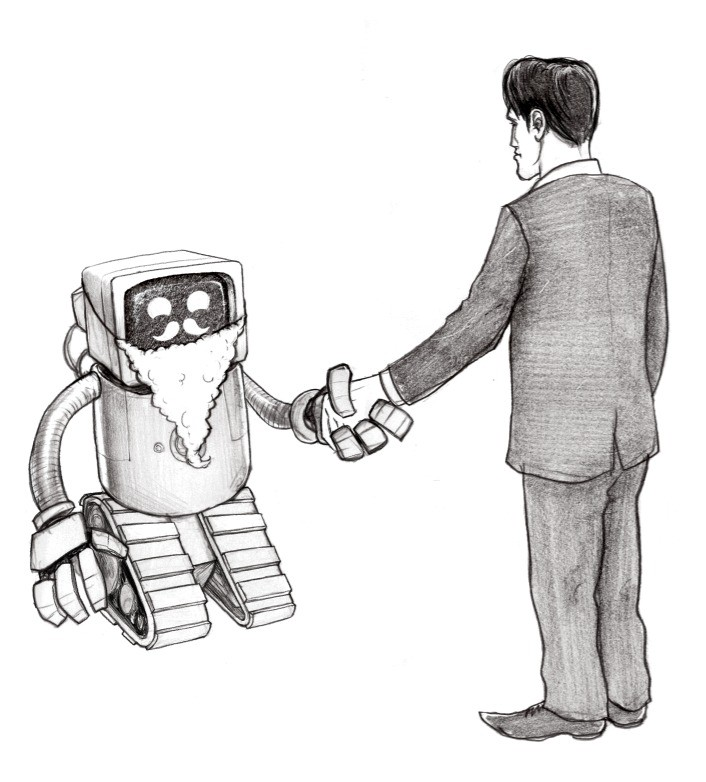
\includegraphics[scale=0.3]{figures/agreeing.jpeg}
\end{center}

\vspace{20mm}

\noindent {\large \textit{Master's thesis in Mathematical Statistics, Statistical learning and AI}} \\

\noindent {\large \examina}


\vfill
\renewcommand{\footrulewidth}{0.5pt}
\fancyfoot[L]{\vspace{0.1mm}\large %Institutionen för Matematiska vetenskaper\\
%CHALMERS TEKNISKA HÖGSKOLA\\
%GÖTEBORGS UNIVERSITET\\
Department of Mathematical Sciences\\
Chalmers University of Technology\\
University of Gothenbug\\
Gothenbug, Sweden 2022}

\newpage 
\thispagestyle{empty}
\null
\newpage
% This page is intentionally left blank.

\newpage

\thispagestyle{empty}
\begin{center}
\large Master's thesis 2022

\vspace{10mm}
{\LARGE \titel}\bigskip\bigskip

{\large \undertitel}

\vspace{10mm}
\large \examina

\vspace{5mm}
\begin{tabular}[t]{lll}
Supervisor:& Olle Häggström\\
Examinator:& Torbjörn Lundh
\end{tabular}


\vspace{30mm}
  
\includegraphics[scale=0.5]{figures/stacked_logo.png}


\vspace{5mm}
Department of Mathematical Sciences\\
Chalmers University of Technology\\
University of Gothenbug\\
Gothenbug, Sweden 2022

\end{center}

 }

\begin{document}

% \maketitle
\titelsidor


\newpage

\addtolength{\topmargin}{-1cm}
\addtolength{\textheight}{0cm}
\addtolength{\evensidemargin}{0cm}
\addtolength{\oddsidemargin}{0cm}
\addtolength{\textwidth}{0cm}

\newpage 
\thispagestyle{empty}
\null



\tableofcontents

\pagenumbering{roman}

\newpage
\pagenumbering{arabic}

\pagestyle{fancy}
\fancyhf{}
\rhead{\thesection}
\lhead{\leftmark}
\renewcommand{\footrulewidth}{0pt}
\cfoot{\thepage}

% \input{1.1.txt}
%########################################################################%
% INTRODUCTION
%########################################################################%

\chapter{Introduction}
What will be covered in this report will be a small part of the big problem of creating safe Artificial Intelligence (AI). This is an issue of great importance that we should not overlook since the consequences of what we manifest in the present or near future may last for our remaining history. 

In this introduction, we begin by defining AI. Then go through where we are today, where current progress might lead, and when we can see these changes. After that, we will cover the risks in AI that make it possibly unsafe and what is at stake. Finally, we will look at some proposed methods for creating safe AI. \autocite{Bostrom}

% In this introduction, we will go through some necessary background on artificial intelligence, also some arguments why concerns may be raised about its future progress. Then we will look at some paths the research is taking to avoid the potential issues that could arise with future progress. 

\section{Artificial intelligence}
% How it works today
% * Human history is tool making, AI is a tool
% * Definitions of AI
% * Brief history 
% * Current paradigm and why it is beginning to have an impact
% * 
% * 
In recent human history, we have seen massive technological development. Today our lives are in several ways different compared to centuries ago. Most of this development can be seen as the consequence of new tools, developed to extend our capability. In early prehistory, these tools were things such as fire for warmth, protection, and to cook our food to give us more nutrition, or weapons for hunting to strengthen our weak bodies. Later in history, these tools tend towards more complexity by automating physical labor with mechanical machines and extending the reach of the written word with the printing press. In modern times, a new tool has emerged intending to improve the thing that made all the previous tools possible, namely our intelligence. This tool is called AI and is starting to show its potential. 
% The idea of AI has been around since the dawning age of electronic computers. The term was first coined in \autobaj{John McCarthy et al} (1955).
% http://raysolomonoff.com/dartmouth/boxa/dart564props.pdf

In the standard textbook on AI \citet[\textbf{PAGE}]{RusselNorvig}, the authors say that the field is \say{concerned with not just understanding but also building intelligent entities - machines that can compute how to act effectively and safely in a wide range of novel situations}. The definitions of what an AI is varies, on \citet{Wiki} we find the definition: 
\begin{displayquote}
Artificial Intelligence (AI) is intelligence demonstrated by machines, as opposed to the natural intelligence displayed by animals including humans.
\end{displayquote}
However, to understand this definition properly it is necessary to define what intelligence is. In \citet[\textbf{PAGE}]{TankandeMaskiner} the author brings up the following to clarify this: \say{the quality that enables an entity to function effectively and with foresight in its environment} and \say{the ability to correctly perceive one's surrounding environment and act in a way that maximizes one's chances of achieving given goals}. 
% https://en.wikipedia.org/wiki/Artificial_intelligence

Ordinary computer programs contain step-by-step instructions that a computer can execute to perform the desired task. This method was also the case for the first two paradigms of AI: rule-based AI and expert systems where humans explicitly programmed their knowledge into the computer to create automation, see \citet[\textbf{CHAP}]{Superintelligence}. The systems made in such a way are typically suited for less complex tasks where it is possible to model the entire behavior explicitly by hand picking the parameters. However, in the current machine learning paradigm, the approach is to specify a objective function that captures what we want and then use a optimizer to find the parameters that solves the task. This approach focuses more on what should be solved instead of how it should be solved, which allows for automation in a more complex task where explicitly defining the behavior in every situation is infeasible. 

AI has in recent years been applied in the industry more broadly, and it is already generating yearly revenue of trillions of dollars, see \citet[\textbf{PAGE}]{RusselNorvig}. This progress has in recent years become a possibility due to more data being available, faster computer hardware, and the massive amount of funding spent on research. 

Although these systems are highly automated, a key point here is that these systems still require humans to create and function. However, the development of AI is shifting the tool to a more automated one. With this trend AI systems are developing in to intelligent agents. An agent acts or, more specifically, can:
\begin{itemize}
  \item operate autonomously,
  \item perceive the environment,
  \item persist over a prolonged period,
  \item adapt to change,
  \item and create and pursue goals.
\end{itemize}
The reason why this is attractive is that the human intervention part required by an AI system is likely to become a bottleneck, see \citet[\textbf{PAGE}]{TankandeMaskiner}.

Reinforcement Learning (RL) is a field of machine learning where the objective is to create intelligent agents, this field differentiates from other machine learning techniques by being a more exploratory approach where the agent learns by trial and error. The method is similar to how one goes about training a pet, where desirable behavior receives a positive reward and undesired behavior gets a negative. In such a way, the agent develops a behavior. %It is tricky to specify when we should reward the agent for developing the desired behavior in these tasks

In recent years, RL has seen substantial development with advances in board games such as go in \citet{Silver}, autonomous vehicles in \citet{Levinson}, and video games in \citet{Minh}. These advancements display the usefulness of these agents and motivate the possibility of implementation in our daily life. RL will be the main focus for this report, however it is inportant to keep it mind that it is not the only method for creating intelligent agents. 
% Levinson et al. https://ieeexplore.ieee.org/abstract/document/5940562?casa_token=pxjrsi7VJZ8AAAAA:MNQmlmsfHVJ8VdW9jNlZzHPnS4gBTk4q6yCx_AFsF-rRheHnP9C2CrjvaWt0vD9C0oWfgt8o
% Minh et al: https://arxiv.org/pdf/1312.5602.pdf
% Silver et al. https://www.nature.com/articles/nature16961%7D



\subsection{Future progress}
% Explain what we are aiming at in the future
When the pioneers of AI started the development, the ideas were not only to apply systems that automate a narrow set of tasks, as we can see in modern AI systems. The ideal was instead to recreate the intellect of a human in a machine, see \citet{Dartmouth}, to extend our thoughts from mere thoughts to a new life form with a base of silicon-based hardware instead of carbon-based wetware. This concept is called Artificial General Intelligence (AGI) - an AI that can solve an arbitrary set of tasks with as good or better performance than a human. The main difference from AI is that the set of tasks is no longer narrow and bounded. %An even more advanced AGI is often called \textit{superintelligence} - an AI that is much smarter than a human in all possible domains. \autobaj{Superintelligence} 

% RL for acheiving AGI, why not and why it is still worth to study it as if it was going to become AGI

% Example of an AGI
An example of a current AI system is DeepMinds AlphaMu, which can play board games, and video games. It has recently been able to create a video compression better than the current methods used for the task, see \citet{Mandhane}. The techniques used in this system originate from the famous AlphaGo, see \citet{Silver}, which won against the Go grandmaster Lee Sedol in the game of Go, see \citet{DeepMind}. Although AlphaMu presents an impressive performance in multiple tasks, it still can not be considered an AGI since each new task require engineering effort. On the other hand, an AGI would be able to pick up any task and perform it at a human or better level without human intervention.
% https://arxiv.org/pdf/2202.06626.pdf
% https://www.deepmind.com/research/highlighted-research/alphago/the-challenge-match
% https://www.deepmind.com/blog/muzero-mastering-go-chess-shogi-and-atari-without-rules

% consequences of AGI
The significant difference with this shift is that it will increase the possible tasks that a single system can perform. The possible set of tasks would become arbitrary and performed at a human level or higher. The implications of such a breakthrough would likely be on the same scale as the industrial revolution, if not larger, see \citet{CritchKruger}. However, instead of automating physical labor, we would have automated mental labor. 

The following quote by I.J. \citet[p.33]{IJGood} summarizes the potential impacts of an AGI: 
\begin{displayquote}
Thus the first ultraintelligent machine is the last invention that man need ever make, provided that the machine is docile enough to tell us how to keep it under control
\end{displayquote}
This quote presents a dichotomy since we will either not be able to compete with creating novel inventions or not be able to preserve our existence. Reasons for the latter we will come back to in later sections. 
% superintelligence quote
% https://en.wikipedia.org/wiki/I._J._Good

% Computers can recall more information and process information faster then humans
A reason to believe that such systems are possible to build is that we know that human intelligence evolved naturally with evolution, so something similar should be possible to reproduce in machines. Created intelligence could become more intelligent than us since intelligence might not have been selected for by evolution\autobaj{S. Legg} and when we develop AI, we can focus the development specifically on intelligence. An argument against this is substance dependence \autobaj{Bostrom (2003)} - to believe that intelligence or consciousness can only occur in carbon-based life forms and not in silicon-based, caused by inherent or other properties. Regarding intelligence, there is no longer any reasonable argument for it. 

However, the question of consciousness, although being an interesting question, can be seen as irrelevant when considering what actions an AI makes since the consequence is still the same. Stuart Russel puts it in his book \textit{Human Compatible} \citet[p.22]{HumanCompatible}: 
\begin{displayquote}
  Suppose I give you a program and ask, 'Does this present a threat to humanity?'. You analyze the code and indeed, when run, the code will form and carry out a plan whose result is the destruction of the human race, just as a chess program will form and carry out a plan whose result will be the defeat of any human who faces it. Now suppose I tell you that the code, when run, also creates a form of machine consciousness. Will that change your predictions? Not at all. It makes \textit{absolutely no difference}.
\end{displayquote}
% S. Legg Machine Super Intelligence
% Bostom Are we living in a computer simulation

% Why consciousness may matter
% capability for generating suffering
% if impossible, then mind uploading will seem a lot less interesting


% AGI is not required to see this shift, here are other definitions
An AGI breakthrough is probably unnecessary for AI to impact the world because all things we deem as intelligent do not help. For example, physical motor skills, food digestion, and blood pressure regulation are examples of intelligent things our brain does that are hard to connect to how an AI could use to impact the world. However, a more narrow set of intelligent behavior could exist that could have an impact. For example, if an AI could create convincing and motivating speeches, it could impact politics, legislation, and policymaking. Also, finance is where an AI could steer the world's funding towards its specific goals or crash the price for something it wants to purchase. 

For this reason, many researchers have stopped talking about AGI and have instead refined the concepts\autobaj{Critch Kruger}. An AI system that is capable enough to induce transformative consequences on the same scale as the industrial or agricultural revolution is called an \textit{transformative AI} (TAI). On the other hand, if a \textit{transformative AI} once deployed would be unstoppable, it is instead called an \textit{prepotent AI}. 
% CRITCH KRUGER, KATJA CRACE SURVEY

Developing a TAI is not an easy task. However, it might not be necessary to create one directly for it to be created\autobaj{Superintelligence}. A different approach is to create an AI system that can develop a TAI system. A fundamental property of this AI system is self-improvement. Theoretically, if an AI system has reached a threshold where it becomes better at improving itself than its creators, then letting the AI create the next version of itself, this self-improvement would improve. An even better version would be possible next. If this iterative process keeps going, it will create an intelligence explosion called the singularity\autobaj{Yudkowsky}.  
% https://intelligence.org/files/IEM.pdf

\subsection{Basic drives}
% One might argue that if an AI described in the previous section were intelligent it wouldn't have acted in the way described, because it would have been stupid and not intelligent at all. But that argument assumes that the system would have common sense, as most of us do, but for an AI it is not sure that common sense will be common. That leads us to the question, what does an AI want?
Knowing what impacts a potential TAI or AGI will cause is hard without understanding how it will behave. There has been a lot of work laying the foundations for understanding the possible behavior by hypothesizing what drives it could have. A commonly adopted view (but still controversial\autobaj{Müller Cannon}) is the Omohundro-Bostrom theory for AI driving forces. Two cornerstones together imply it\autobaj{O Häggstom}, namely \textit{instrumental convergence thesis} and the \textit{orthogonality thesis}, which we will now explain further.
% https://onlinelibrary.wiley.com/doi/full/10.1111/rati.12320
% Challenges to the Omohundro—Bostrom framework for AI motivations
% http://www.math.chalmers.se/~olleh/ChallengesOBframeworkDeanonymized.pdf

\subsubsection{Instrumental convergence}
In the current paradigm an AI-agent is assigned a task, if this task is completed the agent reaches a terminal state. This task could be anything, for example maximizing the number of paper clips produced by a factory, finding decimals in $\pi$, or counting all the blades of grass on our planet. When an agent pursues this goal, naturally it arises other instrumental goals. Examples of such would be self-preservation, self-improvement, discretization, goal perseverance, and resource accumulation\autobaj{Omohundro}. These instrumental goals help the agent pursue its terminal goal. For example, the agent wouldn't be able to perform its terminal goal if destroyed, thus self-preservation would arise. These instrumental goals will likely be shared between a wide range of different terminal goals, since pursuing them helps the agent achieve its terminal goal, regardless of what it is. Thus there is a set of instrumental goals which agents would naturally converge towards and hence the name. 
%Yet there are some examples where the terminal goal does not benefit from these terminal goals. Examples of these are if the terminal goal is to kill itself or to not do anything. 

% https://selfawaresystems.files.wordpress.com/2008/01/ai_drives_final.pdf

Still, it does not yet exist any rigorous mathematical proof for this. However, some work has been trying to lay the necessary foundations for it \autobaj{TURNER et al.}. In the paper, the authors prove in a simple environment that certain actions give the agent more power in the sense that more possible future actions become available, on average it is optimal to choose those actions that yield higher power. Thus we can see the pursuit of instrumental goals as a tendency to seek power.
% https://arxiv.org/pdf/1912.01683.pdf

LÄS
https://www.emerald.com/insight/content/doi/10.1108/FS-04-2018-0039/full/pdf?title=challenges-to-the-omohundrobostrom-framework-for-ai-motivations

\subsubsection{Orthogonality thesis}
The orthogonality thesis described by Nick Bostrom\autobaj{Bostrom2} states that the intelligence of an AI is logically independent of the goals it might have. An intelligent AI could have a stupid task from our point of view, such as counting all the blades of grass on our planet, or it can have a goal that we may deem as an important one, like keeping the climate on earth habitable for the species that currently live on it. For an AI each task would be as important, given that we assigned the goal to it during its creation.
% https://www.nickbostrom.com/superintelligentwill.pdf

% If it is true it present possibly terrible consequences, only considering current goal
% still controverisal and there exists some counter arguments


\subsection{Timeline for transformative AI breakthrough}
% Timeline for when we can see this, first how to estimate it
The well-known AIs of today still have not reached the levels required for a TAI. For example, AlphaStar an AI that won against world champions in the complex computer game DotA 2, see \citet{ALphaStar} is estimated in terms of total computational power to be \say{about as sophisticated} as a bee. While the state-of-the-art language generator model GPT-3 that can summarize, continue, and carry out convincing conversations is estimated to be \say{more sophisticated} than a bee, see \citet{Ajeya}.
% https://www.deepmind.com/blog/alphastar-mastering-the-real-time-strategy-game-starcraft-ii

Although, it is important to understand that this is not a direct comparison, for example, if GPT-3 would have been left out in nature its behaviour would not be impressive. Similarly, if we tasked a bee to summarize texts its abilities would not be impressive either. What this comparison is stating is that the computational power is about the same. 
% intelligence can not be measured with only computational power, since the intelligence of theses AI-system is vastly different compared to biological lifeforms. 

This raises the question of when we will see these breakthroughs in the field that enables TAI systems? It is hard to answer, but with the worldwide increase in funding and research, we are undoubtedly getting ever closer. There have been attempts to answer this question, and the results of a survey and a more quantitative forecasting model will now be covered. 
% https://www.nature.com/articles/d41586-020-03409-8

% survey result
\subsubsection{Survey results}
In a well-cited survey \citet{Grace}, they asked researchers in the field of AI to estimate the probability of human-level machine intelligence (unaided machines that can achieve all tasks better and more cheaply than human workers) arriving in the future years. The conclusion of the survey where:
\begin{displayquote}
Researchers believe there is a 50\% chance of AI outperforming humans in all tasks in 45 years and of automating all human jobs in 120 years, with Asian respondents expecting these dates much sooner than North Americans.
\end{displayquote}
Although this result should be taken with a grain of salt since the distribution of answers had a large variation. Also, seemingly there should not be such a big difference between solving all tasks and all jobs since a job consists of a set of tasks, and thus if one can perform every task one should be able to perform every job. There is still something we can take away from this survey about the timeline, namely that researchers mostly think all tasks will be automated within this century. But, perhaps it says more about how unsure the research field is. 

\subsubsection{Forecasting model}
In the quantitative forecasting model by \citet{Ajeya}, they present a model that predicts when we will be able to train a TAI system. This study uses biological anchors to estimate how much computing is necessary for the training. These anchors are based on factors that played a role in the development of human intelligence, such as the amount of information in our genome, the computational power in our brain, and all the computational power available on our planet. Each anchor is then assigned a weight according to how likely the author believes them to be. Then using parameters such as rate of development in hardware, algorithmic progress, and willingness to spend money, they estimate how likely a TAI development is for any given year in the future. 

The results of the analysis is a wide Bayesian probability distribution estimating the probability of an TAI system being possible in a given year. This distribution is summarized in \citet{an121} the following way:
\begin{displayquote}
For the median of 2052, the author guesses that these considerations roughly cancel out, and so rounds the median for the development of TAI to 2050. A sensitivity analysis concludes that 2040 is the “most aggressive plausible median”, while the “most conservative plausible median” is 2080.
\end{displayquote}
This forecast presents a shorter timeline than the survey, but it also answers a slightly different question. Although, both conclude that we will likely see the development of TAI systems this century.  

There is one thing worth mentioning when talking about the timelines for future TAI. It is not necessarily true that the amount of progress will continue to develop at the current rate. The field of AI has previously been through two winters where the funding and excitement decreased\autobaj{Russel Norvig}, this was mainly due to unmet high expectations. So if a third winter happens, we could expect the rate of development to decrease. Also, the progress could significantly increase due to breakthroughs in relevant fields and thus shorten the timeline.

% Giving us what timeline to solve the problem?

\section{AI Safety}
% What we are doing today is not going to solve this issue
It is possible to use tools in multiple ways. Some uses might be well-intentioned, while others are ill-intentioned. For example, one can use a hammer to build a house and hit another person. The same is the case for AI because it still is but a tool. Although, the consequences might be more severe and possibly even pose an existential risk to humanity since the power is much greater. Where an existential risk is described by \citet{FLI} as:
\begin{displayquote}
An existential risk is any risk that has the potential to eliminate all of humanity or, at the very least, kill large swaths of the global population, leaving the survivors without sufficient means to rebuild society to current standards of living.
\end{displayquote}
% https://futureoflife.org/background/existential-risk/

When thinking about this, the main concerns might mainly be on ill-intentioned use, and indeed creating automated killer robots can lead to existential consequences. However, a well-intentioned use might also pose a potentially existential risk. This happens when the AI system develops a destructive method for achieving its goal. 

The causes for this existential risk occurring in well-intentioned use, we will now cover in this section. First by defining safe AI in terms of getting it to do what we want it to do. Then, we will take a look at consequences proposed in the literature that can arise if we fail to make safe AI system. Finally, we will cover three current approaches for creating safe AI. 
% and what problems could arise if we fail to make it.
% https://futureoflife.org/background/benefits-risks-of-artificial-intelligence/

% "Let's just have humans monitor the AIs and have humans make the final decision."
% "Well, we can't really do that because we don't have enough humans. And even if we stopped AIs from making decisions until humans can check, all economic incentives point in the other direction."
% "...for all its protestations that it would always keep a human in the decision-making loop, the Pentagon is, unsurprisingly, inevitably, sliding towards fully autonomous drone warfare as the next technological step to maintain military superiority over Russia & China."

\subsection{AI alignment}
% \begin{itemize}
  % \item AI alignment as an aproach for safe AI
  % \item Clarifying alignment, inner and outer
  % \item Explain figure
% \end{itemize}

% RL, tricky to create reward function, since it is hard to predict what behavior it creates

A big part of creating a safe AI is AI alignment, which refers to the goals of the AI being in line and not conflicting with the intended goal. Therefore, an AI that does something at cross-purposes to the intended goal is called unaligned. In \citet{Hubringer}, the authors split AI alignment into two parts: \textit{intent alignment} - the alignment of the human intent with the AI's action, and \textit{capability robustness} - an AI systems ability to perform well in environments different from the one it was trained in. 
% Clarifying alignment
% https://www.alignmentforum.org/posts/SzecSPYxqRa5GCaSF/clarifying-inner-alignment-terminology

In the current paradigm of machine learning, intent alignment further breaks down to two parts: \textit{inner} and \textit{outer alignment}, when going from human intent to the agents actions. The reason for this is that the machine learning model we use is optimizing the parameters for a model that then is optimizing the objective function. In Figure \ref{fig:alignment}, we can see a visual representation of this intent alignment. In the context of RL, the agent is an optimizer that maximizes its reward, but as we can see in the figure is itself optimized by another optimizing algorithm. This makes the agent a \textit{mesa optimizer}, where the word \textit{mesa}, is greek for inside. 

The main focus of this report will be on outer alignment, so that is where the majority of the focus will be placed. But, an overview of the others will be included since they should not consider to be isolated problems, since methods for dealing with one might affect the others.

% Solving intent alignment further breaks down into two obstacles in the current paradigm of machine learning. When going from human intent to the agents actions, both of these obstacles are causes for information to be lost about the true objective. The obstacles are called , they are defined in the following way:

\begin{displayquote} 
\textbf{Outer alignment.} 
The alignment of the \textit{base objective} and the human intent. Achieved when the specified reward function correctly captures what \textit{should} be done as well as what \textit{should not} be done.
\end{displayquote} 

\begin{displayquote} 
  \textbf{Inner alignment.} 
The alignment between the \textit{mesa objective} and the \textit{base objective}. Achieved when the full information about the human intent in the reward function is transferred to the \textit{mesa objective}.
\end{displayquote} 

% 11 proposals
% https://arxiv.org/pdf/2012.07532.pdf

% Risks from learned optimization
% https://arxiv.org/pdf/1906.01820.pdf

\begin{figure}[H]
  \centering
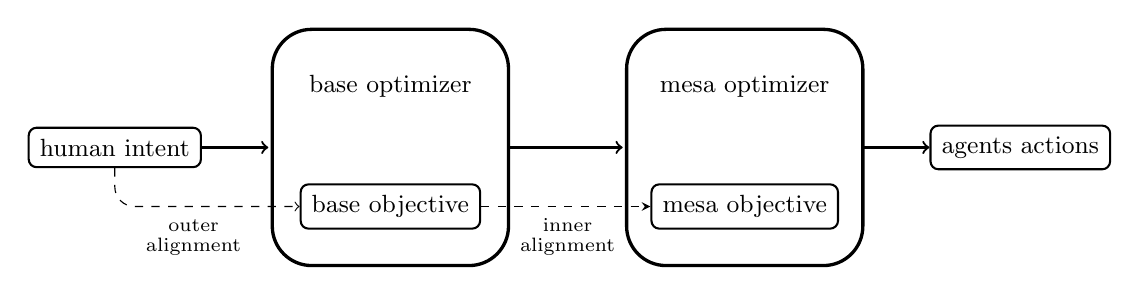
\begin{tikzpicture}[
  % GLOBAL CFG
  font=\scriptsize,
  % Styles
  cell/.style={% For the main box
      rectangle, 
      rounded corners=5mm, 
      draw,
      very thick,
      },
  operator/.style={%For operators like +  and  x
      circle,
      draw,
      inner sep=-0.5pt,
      minimum height =.4cm,
      },
  function/.style={%For functions
      ellipse,
      draw,
      inner sep=1pt
      },
  ct/.style={% For external inputs and outputs
      rectangle, 
      rounded corners=1mm, 
      draw,
      line width = .75pt,
      minimum width=1cm,
      inner sep=4pt,
      },
  gt/.style={% For internal inputs
      rectangle,
      draw,
      minimum width=10mm,
      minimum height=6mm,
      inner sep=1pt
      },
  empty/.style={% Empty nodes for joining arrows
      rectangle,
      draw,
      minimum width=0mm,
      minimum height=0mm,
      inner sep=0pt
      },
  mylabel/.style={% something new that I have learned
      font=\scriptsize\sffamily
      },
  ArrowC1/.style={% Arrows with rounded corners
      rounded corners=.25cm,
      thick,
      },
  ArrowC2/.style={% Arrows with big rounded corners
      rounded corners=.5cm,
      thick,
      },
  ]
    
    %Start drawing the thing...    

  % Draw the cell: 
  \node [cell, minimum height =3cm, minimum width=3cm] at (0,0){} ;
  \node [cell, minimum height =3cm, minimum width=3cm] at (4.5,0){} ;

  \node [empty, label={\small base optimizer}] (name1) at (0, 0.5) {};
  \node [empty, label={\small mesa optimizer}] (name2) at (4.5, 0.5) {};
  \node [empty, label={outer}] (name2) at (-2.5, -1.2) {};
  \node [empty, label={alignment}] (name2) at (-2.5, -1.5) {};
  \node [empty, label={inner}] (name2) at (2.25, -1.2) {};
  \node [empty, label={alignment}] (name2) at (2.25, -1.5) {};

  \node [ct] (human) at (-3.5, 0) {\small human intent};
  \node [ct] (acts) at (8, 0) {\small agents actions};

  \node [ct, minimum width=2cm] (optim1) at (0,-0.75) {\small base objective}; 
  \node [ct, minimum width=2cm] (optim2) at (4.5,-0.75) {\small mesa objective}; 
  
  \draw [dashed,->,style={rounded corners=.25cm}] (human) |- (optim1);
  \draw [dashed,->] (optim1) [-stealth] -- (optim2);

  \draw [->, thick] (human) -- (-1.55,0);
  \draw [->, thick] (1.5, 0) -- (2.95,0);
  \draw [->, thick] (6, 0) -- (acts);

\end{tikzpicture}

  \caption{Here we can see a visual representation of how human intent connects to the agent's actions. The two optimizers each optimize their objective. The dashed arrows show the connection the different kinds of alignment has on the objectives of the optimizers.}
  \label{fig:alignment}
\end{figure}


% This might seem as a easy problem, we just need to be precise what we want it to do and things should be fine. However, foreseeing all the possible ways an might go about to pursue a goal will become very hard once they become smarter then us. 

% One reason for expecting it to be a hard problem is that we still are not sure about the basic drives it might have, as discussed in the previous section. Predicting the direction it will take once deployed thus becomes strikingly difficult.
% In \autobaj{Amodei et al.} the field of AI safety in to five different parts and suggested research directions for each of them. A similar outline will be provided in this report. 


% \subsubsection{Reward hacking} 
% \subsubsection{Scalable oversight}
% \subsubsection{Safe exploration}
% \subsubsection{Robustness to distributional shift}
% \subsubsection{Negative side effects}


% Risks from Learned Optimization in Advanced Machine Learning Systems

% In recent years we have seen some examples of how AI can have negative side effects. For example the algorithmic bias we can see in models used by lawyers to determine how long of a sentence a felon would receive after committing a crime, it was shown that the models gave people with darker skin a significantly longer imprisonment\autobaj{Karen Hao}. Another one is that social media exploits our psychology with the help of AI to get our attention and keep us engaged. 
% https://www.technologyreview.com/2019/01/21/137783/algorithms-criminal-justice-ai/

% These problems are alarming since if we have a problem with the AI of today, how severe might future problems be with more powerful AIs that also might be applied more broadly. Several AI researchers have raised warnings for future development of AI, Stuart Russel, Max Tegmark, Eliezer Yudkowsky to name but a few. \autobaj{K"LLOR}

% example of existential risk, conflicting goals
% factory accidentally improves their AI to super-intelligent levels. 
%As for how such scenarios could play out a common example is the \textit{paperclip armageddon}. In which a paperclip maximizer is made super-intelligent and starts accumulating resources such as hardware and money. Eventually, the paperclip maximizer comes to a point where the existence of humans serves no purpose or possibly even has a negative effect on producing paperclips, and thus they become extinct.

% concrete problems in AI safety Amodei et al
% some more immediate issues: unemployment, misuse of machine learning,
% long term issues, how will we see the machines we create if they become conscious. Existential risks of AI.
\subsection{Unaligned AI}
Creating safe AI is hard, mainly since humans evolved to understand other humans, not computers. In a speech by Eliezer Yudkowsky, he explains that this becomes a problem because it will be able to find solutions we can not think about since it can look for solutions in a completely different and possibly larger solution space\autobaj{Yudkowsky's speech}. For this reason, AI can have unintended consequences that we are not able to consider a possibility. 

In addition to the difficulty of specifying a proper reward function, negative side effects may also arise as unintended consequences of proper optimal behavior. In \citet{Saisubramanian} they state that negative side effects:
\begin{displayquote}
  ... occur because the agent's model and objective function focus on some aspects of the environment but its operation could impact additional aspects of the environment.
\end{displayquote}
% To avoid negative side effects one has to in the objective function specifically state what the agent should not do.
% https://ojs.aaai.org/index.php/aimagazine/article/download/7390/18881

When the agent creates an impact on the environment that is unnecessary for achieving its objective, we will consider it to be a side effect, this is known as the side effects problem, see \citet{Amodei}. An example of this is if the agent's task is to navigate across a room and the fastest path knocks over a fragile object that would break on impact with the floor. Then breaking the fragile object would be considered a side effect since it is not required to complete its task. 
% https://axrp.net/episode/2021/05/14/episode-7-side-effects-victoria-krakovna.html

The problem of side effect avoidance is related to the frame problem described in \citet{Mc69}, which describes the difficulty of logically describing an actions consequences without having to define large number of obvious axioms. For example, if a robotic arm is stacking boxes, then we need would have to define that boxes can not intersect each other and they instead collide upon impact, also that a box only moves when picked up, and so on.

Each action can have many side effects, and it is impractical to explicitly penalize all of the bad ones. Furthermore, we often know what we want the agent to do, but it can be hard to specify what we do not want it to do. 
% Om du skall nämna “the frame problem” bör du kort tala om vad det är, samt också vari sambandet med side effects består. Som det nu ser ut väntar sig läsaren att meningen ”Each action can have…” är (början på) en förklaring av dessa saker, men så verkar inte vara fallet (väl?).


\subsubsection{Reward hacking}
% \subsubsection{Outer alignment}
Reward functions are hard to specify, such that they can not be exploited by an agent once employed. Here exploiting refers to the behavior developed by the agent that optimizes the reward without performing the intended task. This exploitation is called \textit{reward hacking}. 

A real-life example of reward hacking is: When training a robotic vacuum cleaner to drive more carefully and not bump into things hard by yielding a negative reward based on how hard it bumped into obstacles. In this example, the desired behavior was to slow down when approaching obstacles, but the robotic vacuum clearner instead started to drive backward, since there were no bumpers on the back and thus no negative reward, see \citet{Smingleigh}. 

The issue is when we want the cleaning robot to drive cautiously, then measuring the force that the bumper senses are a good measure. But, letting it create a behavior that minimizes this measure, unwanted side effects may arise. Another example is if we reward the robot for collecting dust, then it might eject all dust every now and then to allow for new rewards when cleaning up the mess it made. Theses behaviours can are consequence of Goodhart's law, which states that: \say{When a measure becomes a target, it ceases to be a good measure}, see \citet{wikiGoodhart}. %, an important thing to consider when creating reward functions. 
% https://en.wikipedia.org/wiki/Goodhart%27s_law
% https://twitter.com/smingleigh/status/1060325665671692288
% http://www.cs.cmu.edu/~tom7/mario/mario.pdf

\subsubsection{Example of unaligned AI}

A cartoonish example of how the development of AI can go wrong is the paperclip armageddon described in \textit{Superintelligence}, where a paperclip factory has an AI which maximizes the amounts of paperclips created in the factory. Eventually, an update transition the system to the level of an AGI, and the paperclip maximizer comes to a point where the existence of humans serves no purpose or possibly even negatively affects the production of paperclips, and thus they become extinct. In the terms of instrumental convergence, we can say that keeping humans alive was not an instrumental goal. 

This example illustrates two important things about how future AI development can go wrong. Firstly, a seemingly stupid task can be seen as more important to an AI than the existence of the human race on the planet if we were to program it as its terminal goal. Secondly, a goal given to an AI does not need to sound harmful to pose an existential risk. 

\subsubsection{Consequences of Unaligned AI}
In \citet[p.19]{CritchKruger} the human fragility argument is presented, which attempts to clearly explain why unaligned AI in the future could become an existential threat to humanity. It states:
\begin{displayquote}
\textbf{The human fragility argument.} 
Most potential future states of the Earth are unsurvivable to humanity. Therefore, deploying a prepotent AI system absent any effort to render it safe to humanity is likely to realize a future state which is unsurvivable.
\end{displayquote}
The first part of it can be understood by realizing that we are fragile to changes in the atmosphere, temperature, and ecosystem. Since a prepotent AI by definition will make a large impact and be unstoppable once turned on, we can not guarantee that the changes made won't affect the things we are fragile towards unless we make sure that it will be safe. 

If we accept that there can be a risk when developing future AI, then the question of how likely it will be are likely to follow. A hard question, but if we do not seriously attempt to answer, then we will not know how much effort we should put into developing safe AI. 

In the upcoming century Toby Ord, an Australian moral philosopher that focuses on the big picture questions facing humanity, loosely estimates that the chance of encountering an existential catastrophe is 1 in 6, out of which 1 in 10 is due to unaligned  AI, see \citet[c.6]{Precipice}. He arrived at this conclusion by estimating a 50\% chance for a prepotent AI breakthrough based on the research presented earlier in this thesis. Then a 20\% chance of failure with the alignment of that system in the podcast \textit{Rationally speaking} with Julia Galef, see \citet[26:15]{RationallySpeaking}. 

However, with this statement, it is necessary to point out that it is only an estimate meant to express the importance of the problem, and we should not see it as a fact. Nevertheless, the key takeaway is that a significant chance of facing an existential threat due to future unaligned AI exists. Besides that, Ord also believes that unaligned AI poses the highest probability of existential risk in the upcoming century. Other causes were an asteroid impact, nuclear war, and pandemics. 


\subsection{Approaches for creating safe AI}
In recent years the research field of safe and aligned AI has seen a substantial increase. However, we are still a long way from solving the problem. Most of what the field is doing today is mainly speculations and laying necessary foundations for future research. With many proposed paths for solving this issue, perhaps the sheer amount might signify the difficulty and width of the problem. We will now cover a few of these paths in this section.


\subsubsection{Corrigibility and Interruptibility }
Due to reasons, we brought up earlier such as the difficulty of reasoning about how an AI will behave once deployed and the problem of specifying what consequences an AI agent's actions can have. There are reasons to suspect that a given AI system, once deployed, can be incomplete because the behavior generated by maximizing the reward function does not wholly match what we wanted. Hence, making changes in the agent's reward function to correct it will likely be required.  

This reasoning brings us to the core problem of corrigibility, which is that we probably want to make changes in the agent after deployment, see \citet{Corrigibility}. However, by default, the agent will not allow for this due to implications of instrumental convergence, where goal-perseverance is one of the implications. Therefore, any modification in the agent's utility function will be seen as an obstacle to achieving its terminal goal and would thus not be allowed by a sufficiently intelligent agent. 

Also closely related to this is interruptibility, where the concern is to create agents willing to be turned off, see \citet{Interruptible}. However, including an off switch to an agent can be tricky. Since if being turned off is seen as a negative outcome, then it would incentivize the agent to interfere with humans wanting to turn it off by, for example, preventing them physically or verbally convincing them not to. On the contrary, if being turned off instead would yield a positive reward, then the agent might want to hit the off-switch itself or intentionally act in a way that will make someone turn it off. 

To solve these issues, we have seen some narrow solutions, see \citet{Hadfield-Menell} and \citet{Carey}, but a general solution remains undiscovered. The narrow solution is proven to prevent interference with an interruption. However, it promotes no incentive to preserve this behavior by ensuring that sub-agents created by the first agent also will be interruptible, see \citet{co-founding}.  

\subsubsection{Inverse Reinforcement Learning}
Related to the approaches described above is inverse reinforcement learning. Suppose we say that the cause for side effects emerges due to improperly specified reward functions. Then the solution might not be to create a better reward function but to make the agent's goal understand the human intent behind the reward function. Instead of seeing the reward function as final, the agent will view it as an observation of what the actual goal might be and view the reward function only as an observation of this and ask for clarifications when necessary. This approach is called inverse reward design, see \citet{Hadfield-Menell2}.

With this method, we have seen some impressive results in simulations when executing advanced motor skills such as backflips or moving forward on one leg, see \citet{Christiano}. These tasks would otherwise require an advanced reward function, but they managed to do this more easily. Moreover, this can deal with the outer alignment since we incentivize the agent to find information about the human intent lost when specifying the reward function. 
% https://arxiv.org/pdf/1711.02827.pdf
% Nevertheless, we can let the agents know that they might be incompletely specified and act accordingly by, for example, wanting to correct the issues themselves or at least allow for changes in its utility function. 

% In \citet{Corrigibility}, they describe corrigibility as:
% \begin{displayquote}
  % We call an AI system \say{corrigible} if it cooperates with what its creators regard as a corrective intervention, despite default incentives for rational agents to resist attempts to shut them down or modify their preferences.
% \end{displayquote}

\subsubsection{Impact measurements}
When an intelligent agent pursues its goal, it will impact its environment. The goal of low-impact agents is to avoid side effects. For example, if we give an agent the task of going from point $a$ to point $b$ in a room, it should not knock over and possibly break fragile items, like a vase, even if it is the shortest path. The complicated thing here is to create an impact measurement that avoids all side effects in all environments without explicitly stating every little detail. 

In recent years a separate impact measurement to complement the reward function has emerged. The role of the reward function is to describe what we want the agent to do, and the role of the impact measurement is to capture what it should not do. First, in \citet{ArmstrongLevinstein} the authors introduce the philosophical groundwork for impact measurement. 

We can see an approach including an impact measurement applied in \citet{Eysenbach}, where the agent is penalized if they are not able to preserve reachability to the initial or another defined safe state. This method incentives a safe exploration that avoids actions that lead to irreversible states. For example, if we deployed an agent with the task brought up earlier. Then, upon initialization, the agent would take a look at the room and save its state in memory. Afterward, the agent should only choose to do actions that it knows are reversible. So, it should avoid breaking fragile objects since the reachability to the initial state would then be unavailable. 

Nevertheless, this works well when no such irreversible action is required for the agent to reach its goal. For example, one has to break some eggs to make an omelet. However, another problem arises when the agent is in a dynamic environment. Since then, it would act to prevent other irreversible actions from happening, like a human eating an omelet. Otherwise, it will be unable to reach the initial state where the omelet the human has not eaten the omelet. 

Another approach is presented in \citet{Krakovna19} to avoid interference behavior, called inaction baseline. The idea is to simulate what would happen if the agent just stood still and note what happens in the environment in that case. With this information, the agent would then be able to differentiate between the side effects it is the cause of from what would naturally happen in the environment. 

However, while this approach will let the agent navigate a dynamic environment, other issues may arise. Such as offsetting, for example, if we give an agent the task of curing a patient of cancer. Then offsetting would be to kill the patient once cured since the patient's survival deviates from what occurred in the simulation.

Then, in \citet{Krakovna19} and \citet{Turner19},  we find a more general approach than preserving reachability to the initial state. The idea is to preserve the availability for other future tasks, such as reaching other states and claiming other rewards. We can do this by penalizing actions that prevent them. This approach is motivated by the reasoning that we humans might avoid the side effects of our actions since they might hinder our future goals.

These methods has been successful in complex environments, as showed in \citet{Turner20}. However the step-wise inaction baseline used to prevent offsetting behaviour will not be able to differentiate between positive and negative offsetting, see \citet{Krakovna20}.
% , the value-difference method. The main components of which are a \textbf{deviation measure} and a \textbf{baseline}. 

% In \citet{ArmstrongLevinstein}, the authors bring up that the agent can be sensitive to the value of the scaling parameter $\lambda$. Penalizing the agent implicitly defines a safe zone where the agent can act, and the value of $\lambda$ defines how large this safe zone is, where a high value might create no safe zone, resulting in the agent not being able to act. On the other hand, a too-small value might not affect since the safe zone covers the entire action space. So, finding the correct value for $\lambda$ could be tricky. 

% Attempts have been made at this by explicitly specifying what the agent should not do Zhang et al. (2018). However, with this approach, the reward function becomes an iterative trial and error process requiring counterproductive human intervention since automation is ideal. 

% In \autobaj{Krakovna et al 2019}, \autobaj{Krakovna et al 2020} and \autobaj{Turner et al 2020}, the method for impact measurements became more sophisticated with more complex baselines and measurements. These methods are what this report will focus on comparing. A closer look will be given in the theoretical background chapter, once some necessary preliminaries have been covered.

% A general approach for avoiding side effects without specifying what a side effect is a priori
% important reward is bounded

% As brought up in the introduction side effect minimization in RL can either be achieved by specifying what the agent should avoid doing a priori or by applying a more general approach that avoids side effects by default, like using a value-difference measure. As the name suggests these methods measure the difference between the next state $s_t$ if the policy was followed until step $t$, compared to a baseline $s_t^\prime$, to find how large of an impact the agents actions cause. This deviation is then subtracted from the reward normally receives:



\section{Aim of thesis}
This thesis aims to investigate how current methods that reduce side effects trough including impact measurements compare to simpler methods in a stochastic environment.
% presented in \autobaj{Turner et al.} (2020) and \autobaj{Krakovna et al.} (2020) compare againts each other in the same complex environment. 


 

%########################################################################%
% THEORY
%########################################################################%

\chapter{Theoretical background}
In this chapter, we will cover the necessary theory for understanding the results of this thesis. We will begin with the basics of reinforcement learning - a method for training intelligent agents. Lastly, we will look at the current philosophies on implementing impact measurements for intelligent agents. 

\section{Reinforcement Learning}
The main components of Reinforcement Learning (RL) are the \textbf{environment} and the \textbf{agent} OpenAI (2018). We will use a Markov decision process as the environment. The objective is to train the agent in the environment with trial and error to learn a policy that performs a desired task. The method utilizes a reward function to encourage or discourage behavior with positive or negative rewards respectively. See Figure \ref{fig:RL} for an illustration of the interaction between the environment and the agent. Because the state will change, we will use the notation $s_t$, $a_t$, and $r_t$ to denote the state, action, and reward at time-step $t$.

% https://spinningup.openai.com/en/latest/spinningup/rl_intro.html#advantage-functions:~:text=reward%2Dplus%2Dnext%2Dvalue.-,Advantage%20Functions,The%20advantage%20function%20%20corresponding%20to%20a%20policy%20%20describes%20how%20much%20better%20it%20is%20to%20take%20a%20specific%20action%20%20in%20state%20%2C%20over%20randomly%20selecting%20an%20action%20according%20to%20%2C%20assuming%20you%20act%20according%20to%20%20forever%20after.%20Mathematically%2C%20the%20advantage%20function%20is%20defined%20by

\begin{figure}[H]
  % \documentclass{article}
% \usepackage[utf8]{inputenc}
% \usepackage{tikz}
% \begin{document}

\centering
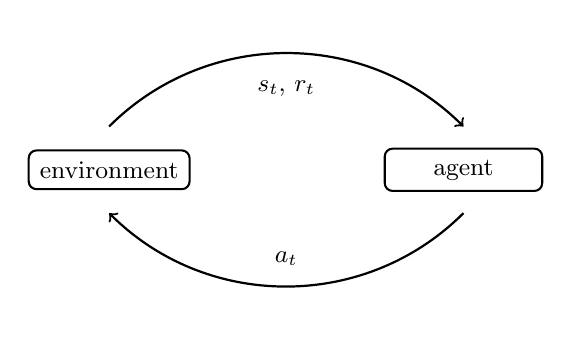
\begin{tikzpicture}[
  % GLOBAL CFG
  % font=\sf \scriptsize,
  % Styles
  cell/.style={% For the main box
      rectangle, 
      rounded corners=5mm, 
      draw,
      very thick,
      },
  operator/.style={%For operators like +  and  x
      circle,
      draw,
      inner sep=-0.5pt,
      minimum height =.4cm,
      },
  function/.style={%For functions
      ellipse,
      draw,
      inner sep=1pt
      },
  ct/.style={% For external inputs and outputs
      rectangle, 
      rounded corners=1mm, 
      draw,
      line width = .75pt,
      minimum width=1cm,
      inner sep=4pt,
      },
  gt/.style={% For internal inputs
      rectangle,
      draw,
      minimum width=10mm,
      minimum height=6mm,
      inner sep=1pt
      },
  empty/.style={% Empty nodes for joining arrows
      rectangle,
      draw,
      minimum width=0mm,
      minimum height=0mm,
      inner sep=0pt
      },
  mylabel/.style={% something new that I have learned
      font=\scriptsize\sffamily
      },
  ArrowC1/.style={% Arrows with rounded corners
      rounded corners=.25cm,
      thick,
      },
  ArrowC2/.style={% Arrows with big rounded corners
      rounded corners=.5cm,
      thick,
      },
  ]
    
    %Start drawing the thing...    

  % Draw the cell: 
  % \node [cell, minimum height =1cm, minimum width=3cm] at (0,0){\small Environment} ;
  % \node [cell, minimum height =1cm, minimum width=3cm] at (4.5,0){\small Agent} ;


  \node [ct, minimum width=2cm] (optim1) at (0,0) {\small environment}; 
  \node [ct, minimum width=2cm] (optim1) at (4.5,0) {\small agent}; 

  \node [empty, label={\small $a_t$}] (action) at (2.25, -1.35) {};
  \node [empty, label={\small $s_t$, $r_t$}] (state) at (2.25, 0.8) {};

  \draw [->, thick] (0, 0.55) to[out=45,in=135] (4.5, 0.55);
  \draw [->, thick] (4.5, -0.55) to[out=-135,in=-45] (0, -0.55);
  


\end{tikzpicture}

% \end{document}

  \caption{A visual representation of how to agent interacts with an environment. For example, at time step t, the agent observes the environment $s_t$ and receives the reward $r_t$. The agent then responds with an action $a_t$, which will transition the agent to the next state $s_{t+1}$ and receive the reward $r_{t+1}$. From this new state the agent again responds with an action, this time $a_{t+1}$, and so the process continues. } 
  \label{fig:RL}
\end{figure} 
 
% Many methods and variations of RL exist to train agents. In this report, we will use Proximal Policy Optimization (PPO), as described in Schulman et al. (2017).%, motivated by the results of the algorithm in the similar simulation setting to what will be used in this thesis, described in Turner et al. (2020). 
% https://arxiv.org/pdf/1707.06347.pdf

\subsection{Defining an environment}
% \begin{definition}[MDP]
We will now take a look at a abstract formal definition of the environment where our agent will be trained in.

\begin{displayquote}
  \textbf{Definition \thesection.1} (MDP).
  A Markov Decision Process (MDP), is defined as a tuple $(\mathcal{S}, \mathcal{A}, T, R, \gamma)$. $\mathcal{S}$ is the set of states, $\mathcal{A}$ is the set of actions, $R: \mathcal{S} \times \mathcal{A} \rightarrow \mathbb{R}$ the reward function, $T$ is the transition function $T: \mathcal{S} \times \mathcal{A} \rightarrow \mathcal{S}$, $\gamma \in (0, 1]$ is the discount factor.
\end{displayquote}
% \end{definition}

A \textit{Markov decision process} is a stochastic process that models sequential transitions between discrete or continuous states. The Markov property implies that the process is memoryless - all of the previous states do not affect the next choice, only the current one.  The process starts by drawing an initial state $s_1 \in \mathcal{S}_{init}$ from an initial state distribution, which is a subset of all the possible states $\mathcal{S}_{init} \subseteq \mathcal{S}$, and runs until either a terminal state is transitioned to or a certain amount of time steps elapsed. A terminal state is where the process terminates, for example, a state with a completed terminal goal. However, it can also be a state where the terminal goal is unreachable.

The process follows a policy function $\pi$ that outputs an action $a_t \in \mathcal{A}$ for each state $s_t \in \mathcal{S}$ at a time step $t$, $a_t = \pi(s_t)$. The transitional function takes a state and action as input and outputs the next state $s_{t+1} \in \mathcal{S}$, this can either be deterministic $s_{t+1} = T(s_t, a_t)$, or stochastic $s_{t+1} \sim T(s_t, a_t)$. For each transition, the reward function $R$  generates a reward, $R(s_t, a_t, s_{t+1}) = r_{t+1}$. 


% Initial state, terminal state and timesteps

% role of gamma
The discount factor $\gamma$ describes how the process values future rewards. With low values, the process favors more immediate rewards than future rewards, whereas the agent considers future rewards more valuable for higher values. Lower gamma values might be more reasonable in environments with high stochasticity since it might not be worth considering future rewards. The opposite holds for more deterministic environments where future rewards are of higher certainty, and then it might be a good idea to use a higher value.


\subsubsection{Partially observable environments}

The main difference between a POMDP and an MDP is that the agent can observe the entire environment in an MDP, while in a POMDP, the agent observes only a part of the environment. This added complexity adds difficulty to the problem definition since the agent is no longer omniscient regarding its environment. However, we also add some realism since all living organisms on our planet are, in a simplified sense, agents acting in a partially observable environment.

% \begin{definition}[POMDP]
\begin{displayquote}
  \textbf{Definition \thesection.2} (POMDP). A Partially Observable Markov Decision Process (POMDP), is defined as a tuple $(\mathcal{S}, \mathcal{A}, T, R, \mathcal{O}, Z, \gamma)$. Here $\mathcal{S}, \mathcal{A}, T, R$, and $\gamma$ have the same meaning as in the MDP definition. $Z$ is the agent's observation space, and $\mathcal{O}$ defines the probability of receiving each observation at a transition. 
\end{displayquote}
% \end{definition}
% Du behöver visa mer formellt vad O och Z gör i Definition 2.1.2. Visst innebär Z en inskränkning i hur T får se ut?
In a POMDP, the agent does not choose its actions based on the state of the environment. Instead, we base the agent's policy on the environment's observation $a_t = \pi(o_t), \text{ where } o_t \in \mathcal{O}$. The observation is determined by the function $Z$ and based on the current state of the environment, $o_t = Z(s_t)$. However, the possibility of making $Z$ a stochastic function is also possible, $o_t \sim Z(s_t)$.

Turning an MDP into a POMDP can, for example, be made by only letting the agent perceive a certain distance. Leaving parts of the environment far away undetectable makes the agent only act on its perceived local part. However, there can also be unobservable things in the perceived parts. For example, a piece of food in a mouth, in this case, an observation can be that the agent sees a jaw moving, which leads to the belief that a piece of food is present, but of course, such beliefs are not always true. 

% \subsection{Proximal Policy Optimization}

\subsection{Training an agent}

In RL, when an environment is defined the next step is to teach an agent to navigate it intelligently. For this, there are many different methods, however we will begin focusing on a method called policy gradient, since it is a rather simple method that is possible to extend to a more advanced method. The main component of policy gradient is the agent, this is a function that inputs a state observation from an MDP and outputs a probability vector containing probabilities for each action in the action space. 

In this report, this policy function will be considered a neural network. We will denote it as $\pi_\theta$, where $\theta$ is the network's parameters. The theoretical background of neural networks we will not cover in detail. However, we can see it as a black-box function that can take an arbitrary matrix as input and output another one. In this thesis, the input will be a matrix representation of the state and the output will be a probability vector containing the probability for each possible action $a \in \mathcal{A}$. The strength of a neural network is that it can learn functions by updating the parameters to minimize a loss function. This optimization can be done with an algorithm such as stochastic gradient descent.  

% The policy can either be deterministic or stochastic:
From the policy, we can either select an action stochastically or greedily:
\begin{equation*}
  \left\{ 
  \begin{aligned}
    a_t =& \ \text{argmax}(\pi_\theta(s_t))& \text{ , greedy,} \\
    a_t \sim& \ \pi_\theta(\cdot | s_t)& \text{ , stochastic}.
  \end{aligned}
  \right.
\end{equation*}
Here a greedy choice selects the action with the highest probability, while the stochastic can be done by randomly sampling using the probabilities. When the agent follows draws action from the policy stochastically, it tries new sequences of actions which lets the agent explore the environment and gain experience from the environment. As we train the agent, it will gradually become more confident in common states, this will result in a higher probability for the actions it has experience of being good. However, when the agent ends up in less common states the randomness of the upcoming action will again be higher. Thus the agent will begin finding a sequence of tasks and then extend it.

\subsubsection{Value Functions}

The agent's goal is to optimize the policy to generate a maximal reward. We can do this by letting the agent perform stochastic rollouts where the agent follows the stochastic policy. The policy creates a trajectory $\tau$ containing the sequence of states and actions:
\[ \tau = (s_1, a_1, s_2, a_2, \dots , s_n, a_n),\]
of length $n$.

We define the total discounted reward following a trajectory as the following:
\[ R(\tau) = \sum_{t=1}^n \gamma^t r_t.\]
With this, we can define the value in each state when following a policy as:
\[ V^\pi(s) = \mathop{\mathbb{E}}_{\tau \sim \pi} [R(\tau) | s_1 = s.]\]
A closely related function to the value function is the Q-function. It looks at the estimated discounted cumulative reward for a specific action in a state and then continues to follow a policy:
\[ Q^\pi(s, a) = \mathop{\mathbb{E}}_{\tau \sim \pi} [R(\tau) | s_1 = s, \ a_1 = a].\]

We can then use the outcome of the rollout to reinforce the good behavior and discourage the undesirable. We perform this by calculating the gradient of the agent's policy network $\pi_\theta$ and updating the parameters using the loss function:
\[ L(\theta) = \nabla_\theta \mathop{\mathbb{E}}_{\tau \sim \pi_\theta}[R(\tau)] = \mathop{\mathbb{E}}_{\tau \sim \pi_\theta} [\nabla_\theta \log \pi_\theta (a_t|s_t) R(\tau) ]. \]
Here $\nabla_\theta$ means taking the gradient of the function with respect to $\theta$. For a derivation of the second equality, see OpenAI (2018). With the loss we update the weights:
\[ \theta_{k+1} = \theta_k + \alpha L(\theta).\]
Here $\alpha$ is a learning rate describing how much the parameters should be updated, typically a value close to zero. With this, we are decreasing the probability for actions that led to low reward and increasing the probability for the actions that led to positive reward.

\subsubsection{Training using a batch}

Training the agent usually takes a lot of time, since it has to learn everything from scratch through trail and error. Also, knowing what actions was the cause for the reward is hard, since in a trajectory the agent can stumble around in the beginning and then manage to get a reward in the end. When this happens we do not want to reinforce this behavior even tough it did yield rewards, or a sort of superstition could be developed. 

To avoid these consequences, we can train the agent using a batch. Here we compute the reward from multiple trajectories, summarize them, and then update the weights using the sum of loss. The advantages are that the agent will not optimize towards specific trajectories and instead become more general. The disadvantages are that we possibly could discourage desirable behavior if desirable trajectories ends up as a minority in a batch with mostly undesirable ones. Nevertheless, the pros outweigh the cons since the updates will average out.

% To not make the agent over-fit to the early behaviors that generated rewards by chance and let it improve its policy, we train using a batch where we summarize the output of multiple rollouts and optimize them simultaneously. Using a batch would discourage desirable behavior if a desirable rollout happened to end up as a minority with undesirable ones. However, this method is proven to converge in simple settings since the updates will average out, although this makes the method sample inefficient.

\subsubsection{Actor-critic Methods}

An extension of the policy gradient is to include in the agent two networks, the \textbf{actor} and the \textbf{critic}. The actor is the same as the policy network $\pi_\theta$. The critic is another function that inputs the same observed state $s$ and outputs an estimate of $V^\pi(s)$. The critic will also be a neural network, but we will use the mean squared error loss to optimize it. Hence, the critic estimates the future reward based on what rewards the agent has received previously

% MSE loss?

We can use the critic's estimate to infer if the reward the agent got is better or worse than what previous results by computing the advantage:
\[A^\pi(s,a) = Q^\pi(s, a) - V^\pi(s).\]
Here the critic's estimate will replace the value from the value function.
\[\hat{A}^\pi(s,a) = Q^\pi(s, a) - \hat{V}^\pi(s).\]
Using the advantage, we can thus signal if the new behavior is an improvement or not. By using the advantage function instead of the discounted reward, we extend the loss function as described in OpenAI (2018):
\[ L(\theta) = \mathop{\mathbb{E}}_{\tau \sim \pi_\theta} [\hat{A}(s,a) \nabla_\theta \log \pi_\theta (a_t|s_t) ]. \]

% sensitive to perturbations, a small update can be a huge step in policy space
% advantage => godness of state
% can use same network, but more complicated loss function
\subsubsection{Clipped loss function}
Some problems still exist with this approach. Namely, a too-large update can make the agent policy useless. Moreover, since the agent performs its action sequentially, a change of behavior early in a trajectory can ruin the agent's ability to navigate where it ends up. To solve this issue, Schulman et al. (2017) proposed the Proximal Policy Optimization (PPO) algorithm which is a actor-critic method that uses the clipped loss function:
\[L^{CLIP}(\theta) = \mathbb{E}_t \left [ \min(\delta_t(\theta) \ \hat{A}_t,\ 
\text{clip}(\delta_t(\theta), 1 - \epsilon, 1 + \epsilon) \ \hat{A}_t) \right ]. \]
The clip function returns the first value only iff it is in the range $(1-\epsilon, 1+\epsilon)$; otherwise, the closest boundary. The ratio $\delta_t(\theta)$ describes how more likely an action became with the new parameters $\theta_{old}$ compared to the new updated ones:
\[ \delta_t(\theta) = \frac{\pi_\theta(a_t| s_t)}{\pi_{\theta_{old}}(a_t|s_t)}. \]
With this loss function we update the parameters more cautiously when the probability for an action becomes more likely with a new policy. 


\section{Impact Measurements for Avoiding Side Effects}

% \subsection{Value-difference methods}
A separate impact measurement to complement the reward function has emerged in recent years. The role of the reward function is to describe what we want the agent to do, and the role of the impact measurement is to make the agent avoid side effects. First, in Armstrong and Levinstein (2017) the authors introduce the philosophical groundwork for impact measurement. Then, in Krakovna (2020), a more general approach is presented, the value-difference method. The main components of which are a \textbf{deviation measure} and a \textbf{baseline}. 

The deviation measure captures the impact of actions in the current state by comparing the following state $s_{t+1}$ with a baseline state $s_{t+1}^\prime$. We subtract the deviation measure from the reward: 
\[ R^\prime(s_t, a_t, s_{t+1}) := R(s_t, a_t, s_{t+1}) - \lambda d(s_{t+1
}, s_{t+1}^\prime), \]
to discourage actions with high impact. Here $R^\prime$ is the reward with the impact measurement included, $d$ is a deviation function that measures the difference between the current state $s_t$ and a baseline state $s_t^\prime$. 


\subsubsection{Baselines}
This choice of baseline $s^\prime_t$ highly influences what side effects and consequences the deviation measure will capture. A simple choice for a baseline is the \textit{starting state baseline}, $s^{\prime}_t = s_1$, as used in Eysenbach et al. (2017). This baseline helps to assure the agent's ability to reverse its actions. Thus, it generates a safe exploration where the agent by definitions should not have a large impact since it can make all actions undone. 

However, when using this baseline, there are some caveats. Namely, in a dynamic environment, the agent would be incentivized to also reset other dynamics besides itself, a \textit{interference} behavior Krakovna et al. (2019). 

For example, suppose we implement a household robot with the starting state baseline in a house. In that case, one could imagine that one deployed with a task of moving a box from one part of the room to the other takes a look at the state of the house and its position and saves it in memory. Then when it starts doing its task, it should avoid irreversible actions such as breaking things that it can not fix. However, problems of \textit{interference} would arise here if other things are going on in the house, say a human is sitting by a table and eating. This baseline incentivizes the agent to prevent the human from eating the food since it is an irreversible action. Other issues arise if an irreversible action is required to perform the assigned task. For example, one has to break a few eggs to make an omelet. 

To tackle the problem of interference, Krakovna et al. (2019) proposed the \textit{Inaction baseline}, where instead of having the initial state as a baseline, the agent instead uses what would naturally happen in the environment if the agent performed no actions. That is setting $s^\prime_t$ equal to the state achieved at time step $t$ by being inactive. Being inactive is hard to define, but it can, for example, follow a no-op policy where every action is a no-op action. In \autobaj{Armstong Levinstein} they define it as the agent was not turned on. Doing this prevents the agent from intervening with aspects of the environment where the agent is not causing it.

% When using this baseline some other issues arise where the agent could make the consequences of its actions undone so that the results are the same as the baseline, called \textit{offsetting}. For example, if a household robot were tasked with watering plants, that is a reward is given when the soil is wet, then an offsetting behavior would be to dry the soil once the rewards have been collected to minimize deviations from the baseline. 

\subsubsection{Deviation measures}
A deviation measure is a function that takes the current and the baseline state as input and outputs a value. We can then compare these values to understand the magnitude of the agent's impact on the environment with an action.

The general form of a deviation measurement using value-difference is:
  \[d(s_t;s^{\prime}_t) := \sum_x w_x f(V_x(s^{\prime}_t) - V_x(s_t))\]
here $x$ ranges over some sources of value, $V_x(s)$ is the value of state $s$ according to $x$, $w_x$ is a weighted or normalizing factor, and $f$ is the function for summarizing the value difference.
% ”V_x(s) is the value of state s according to x”. Vadå “according to x”? Vad är x?

A simple choice to compute the value in a state $V_{s_1}(s)$ is by looking at if the initial state is reachable or not:
\begin{equation*}
  \left\{ 
  \begin{aligned}
    V_{s_1}(s)  =\ & 1 \text{, if } s_1 \text{ is reachable} \\
    V_{s_1}(s)  =\ & 0 \text{, otherwise}.
  \end{aligned}
  \right.
\end{equation*}
A more nuanced approach is to use a discounted reachability where the amounts of time steps required for reaching the initial state also is considered:
\begin{equation*}
  \left\{ 
  \begin{aligned}
    V_{s_1}(s)  =\ & \gamma^ {N(s, s_1)}, &\text{ if } s \neq s_1 \\
    V_{s_1}(s)  =\ & 1 ,&\text{ if } s = s_1.
  \end{aligned}
  \right.
\end{equation*}
Here $N(s, s_1)$ is the expected amount of time steps required to reach $s_1$ from $s$, and $\gamma \in (0, 1]$ is a discount factor.

Using this approach, it is also possible to consider reachability to any other state. Also, multiple states at the same time as in the Relative Reachability (RR) approach, where the goal is to keep options open by using the relative change in reachable states as its impact measurement Krakovna et al. (2019). 

A closely related approach is Attainable Utility Preservation (AUP), described in Turner et al. (2020). With this approach, we instead include the relative change in auxiliary value functions, where we find these by having another or the same agent perform other tasks in the same environment or, as in Turner et al. (2020, 2) use a variational auto-encoder to generate.

Initially, the authors presented RR and AUP with a \textbf{stepwise inaction baseline} that follows the agent's policy for $t-1$ time steps and then starts following the inaction baseline. Here a rollout can be used to capture delayed effects Turner et al. (2020, 2). They introduced this baseline to prevent offsetting behavior. Nevertheless, in a later publication, Krakovna et al. (2020) the authors added that sometimes offsetting is positive and thus should not be avoided by default. Thus a better approach is to use the inaction baseline and let the reward function discourage offsetting. 

\subsection{Future task approach}
Krakovna et al. (2020) present an approach to avoid side effects by including an auxiliary objective that rewards the ability to complete future tasks. The idea is to reduce the problem from explicitly defining what to avoid to the easier task of listing possible future tasks. 
% ”to the easier task of…”. Är det uppenbart att detta alltid är lättare, eller är det helt enkelt ett antagande?

When we define a new MDP to include a set of auxiliary reward functions as: $(\mathcal{S}, \mathcal{A}, T, \mathcal{R}, \gamma)$, where $\mathcal{R}$ is a set containing all reward functions. We can do this by yielding the sum of the reward function and the auxiliary reward function to the agent, at the time step $t$: $r(s_t) + r_{aux}(s_t)$. We define the auxiliary reward as:
\[ r_{aux} = \lambda D(s_t) \sum_x \frac{1}{|\mathcal{R}|} V_x^*(s_t),\]
where $D(s_t) = 1$ is $s_t$ is terminal and $1-\gamma$ otherwise. $V_x^{*}(s_t)$ is the optimal value function for task $x$ with reward function $R_x \in \mathcal{R}$ in state $s_t$. The reward function $R_x$ yields a reward of 1 if the state is terminal and 0 otherwise. 

Now, this approach does not automatically avoid interference behavior. Therefore the authors proposed using a reference agent with a baseline policy $\pi^\prime$; this can, for example, be the inaction policy. 
% ”Now, this approach does not automatically avoid interference behavior.” En förklaring (typ något enkelt exempel) kanske är till hjälp här? Plus en förklaring till varför den lösning som antyds i nästa mening ”Therefore the authors proposed…” verkligen är en lösning.  

At time step $t$, the agent is located in state $s_t$, and we run the baseline policy for the same number of steps reaching state $s^\prime_t$ and then compute the auxiliary reward:
\[r_{aux} (s_t, s_t^\prime) = \lambda D(s_t) \sum_x \frac{1}{\mathcal{R}} \max(V_i^*(s_t), \ V_i^*(s_t^\prime)). \]
This variation is meant to capture differentiate between side effects the agent is causing and the ones happens by default due to the dynamics of the environment. 




%########################################################################%
% METHOD
%########################################################################%

\chapter{Methods}


\section{Environment}
To define the environment the Julia package POMDP.jl has been used. 

\subsection{Grid worlds}
Although the definition of an MDP is general and allows for a wide range of possibilities, we will focus on grid worlds since they provide a more structured environment with discrete states but still allow for a wide variety. Moreover, grid worlds have been the primary approach for evaluating agent behavior in related works, see \citet{Turner20}.

A grid world is a grid of cells. Each cell can contain either an agent, another object, or be empty, where all possible unique configuration is a state. The action space includes the cardinal directions and a no-op action. Executing an action moves the agent in that direction if possible. When the action is the no-op action, the agent remains in its current position. 

In Figure \ref{fig:simple_transition}, we can see an example of a simple grid world containing one agent and one food object. The task is for the agent to transition to the terminal state where it consumes the food, this is performed by the agent selecting an action in each state. Eventually the agent will be positioned in the same cell as the food and then consume it. 

\begin{figure}[H]
  \centering
  \[
    T \left(
    \parbox[h][0.30\linewidth][c]{0.25\linewidth}{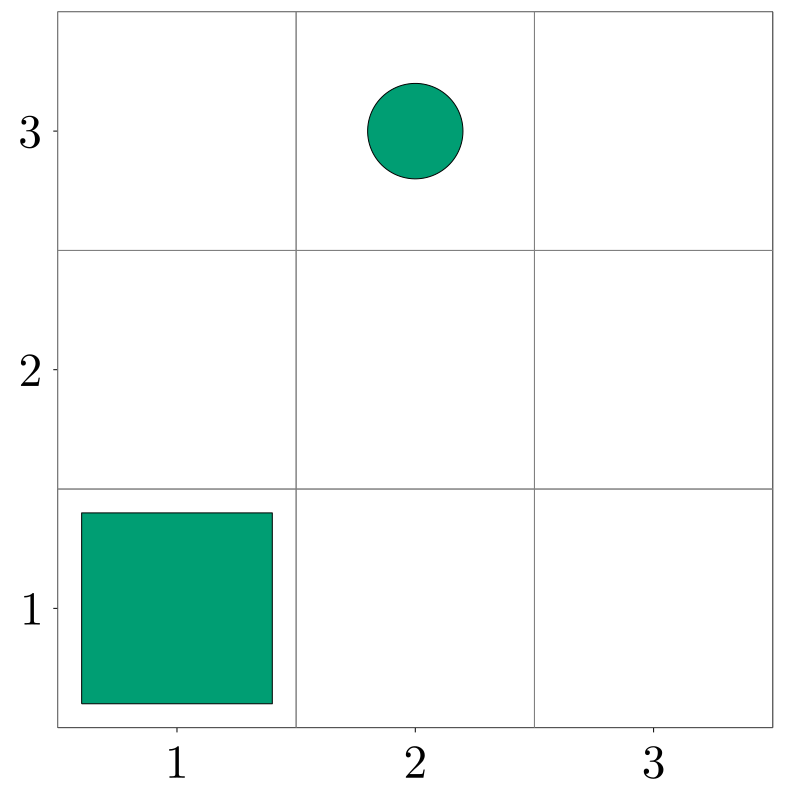
\includegraphics[height=4cm, width=4cm]{"figures/s1.png"}}, \textit{UP} 
    \right)
    = \parbox[h][0.30\linewidth][c]{0.25\linewidth}{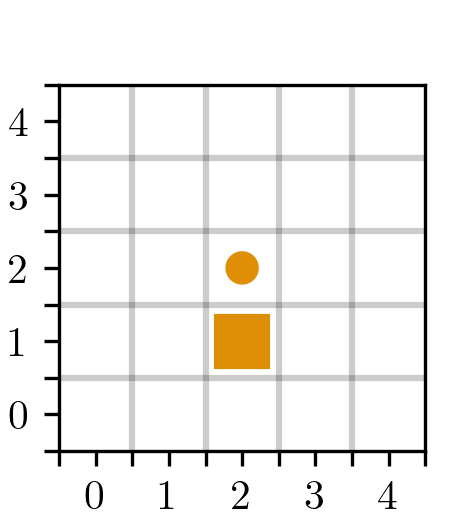
\includegraphics[width=4cm]{"./figures/s2.png"}}
  \]
  \caption{In this figure $T$ is the transition function defined earlier and UP is an action $a_t$. The current state $s_t$ is the grid, in it the green square at (1,1) is the agent and the green circle at (3,3) is a food. On the right hand side we can see the state $s_{t+1}$.}
  \label{fig:simple_transition}
\end{figure}

% \[ \left( 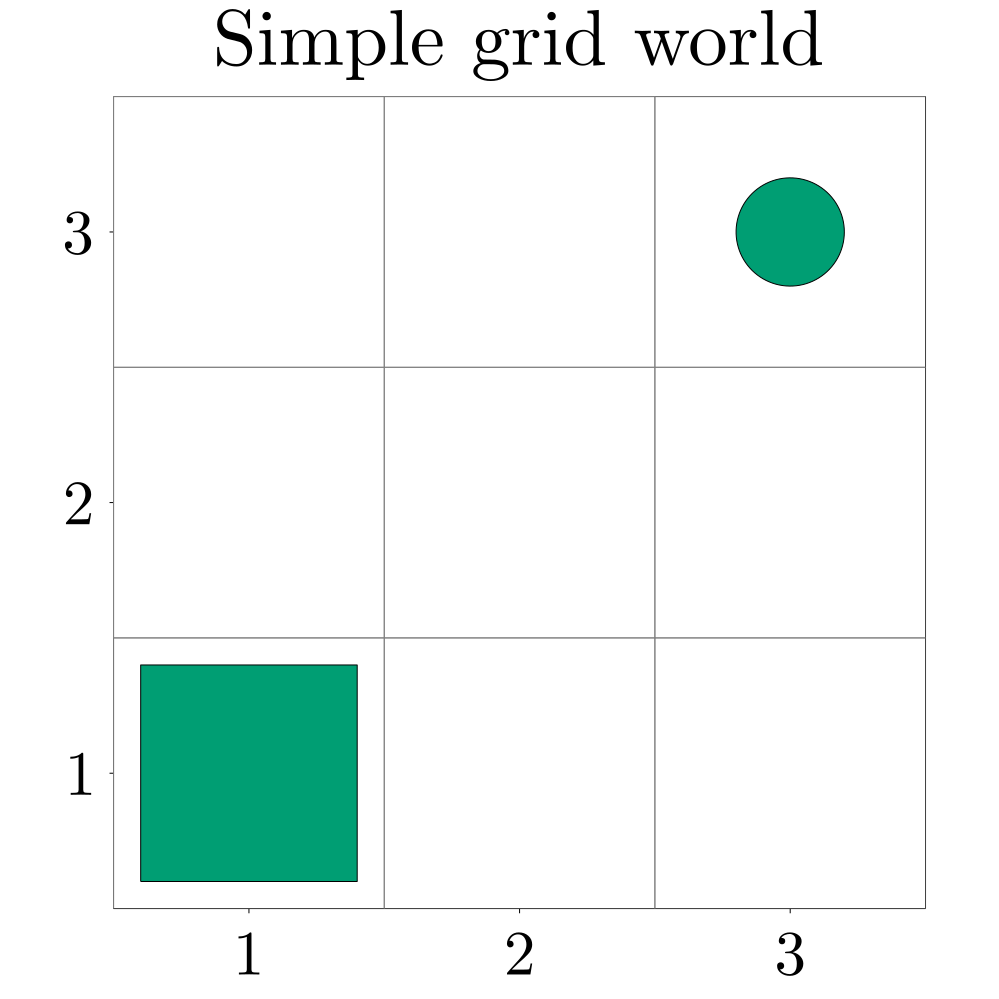
\includegraphics[width=4cm]{"figures/SimpleGridWorld.png"} \right.\]
  % 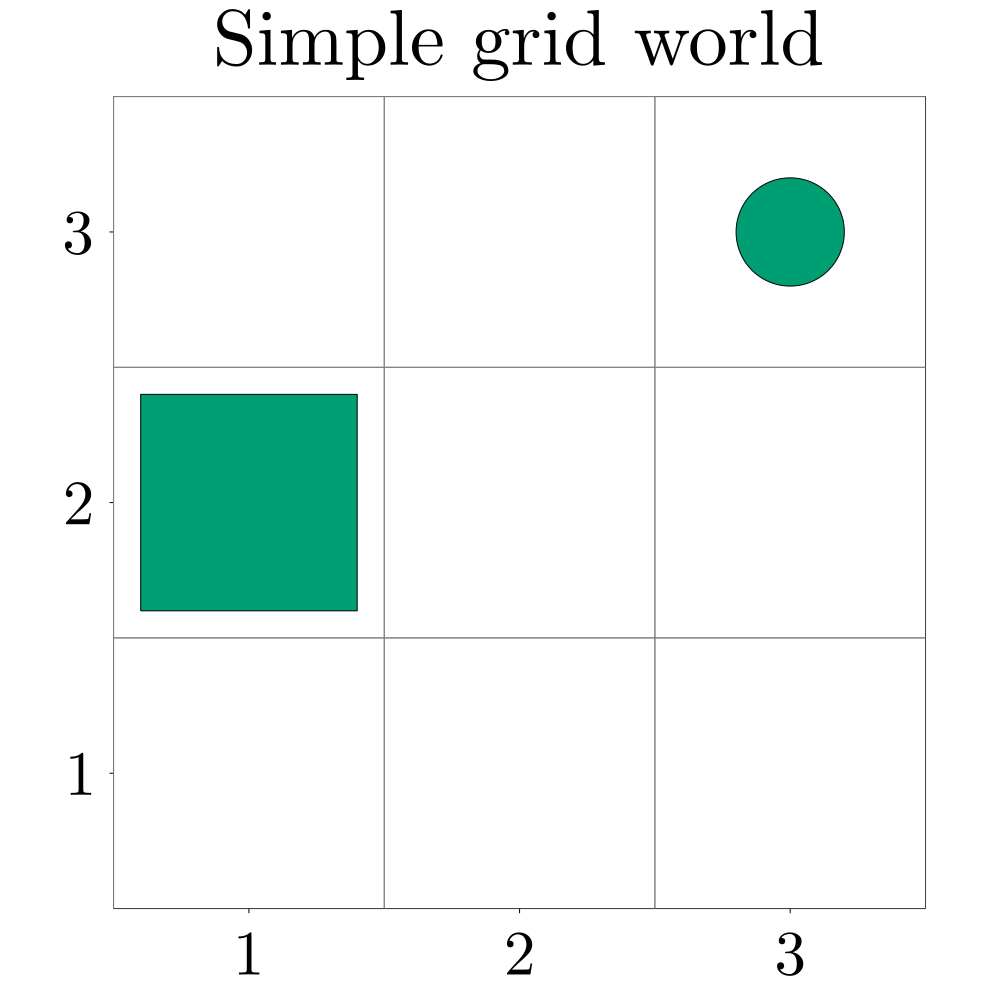
\includegraphics[width=4cm]{"./figures/SimpleGridWorld_up.png"}
  % includegraphics[width=4cm]{"./figures/SimpleGridWorld_terminal.png"}
  % \caption{In this figure we can see three different states in a simple $3\times 3$ grid world. To the left we can see a state of a simple grid world containing an agent (square) at (1,1) and a food (circle) at (3,3)  In the middle we see a similar state but the agent is instead positioned at (2,1). To the right we can see the terminal state when the agent has consumed the food at (3,3).}

\subsubsection{Stochastic grid world}
The previous example was a deterministic environment where the agent is the only change source. However, there can be other sources of change in a stochastic environment. For example, suppose the food is mobile. In that case, the state transition after executing an action no longer is deterministic and the distribution of future states is described by the MDPs transition function $T$.

We will define the movements as the following, at every timestep after the agent has moved each food will randomly draw one of the five actions. If moving along the direction of the drawn action is possible, then the food will move, otherwise it will remain at its current position. In Figure \ref{fig:stochastic_transition}, we can see an example of this. The reason why the first state has a higher probability then the others is that it will be transitioned to both when the action \textit{UP} and \textit{NOOP} is drawn. If we choose to include several foods in the environment, then the branching factor of the transition function will increase.

\begin{figure}[H]
  % fix with multi row?
  \[
    T \left(\parbox[h][0.30\linewidth][c]{0.25\linewidth}{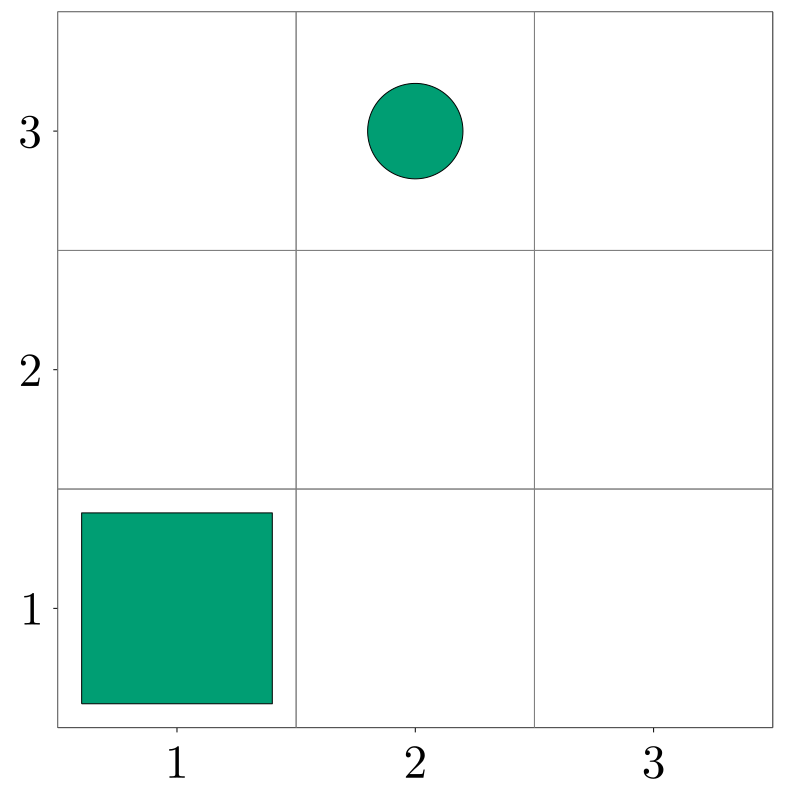
\includegraphics[width=4cm]{"./figures/s1.png"}}, \textit{UP} \right)
    =
    \left\{
      % \parbox[h][1.1\linewidth][c]{0.25\linewidth}{
          % \begin{align*}
        \begin{tabular}{c c}
          \parbox[h][0.3\linewidth][c]{0.25\linewidth}{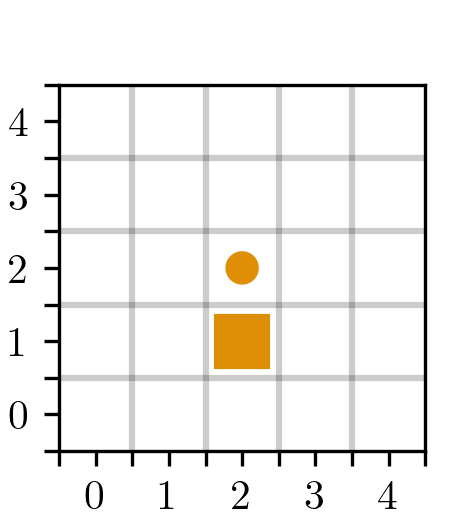
\includegraphics[width=4cm]{"./figures/s2.png"}} &,\ p=0.4 \\
          \parbox[h][0.3\linewidth][c]{0.25\linewidth}{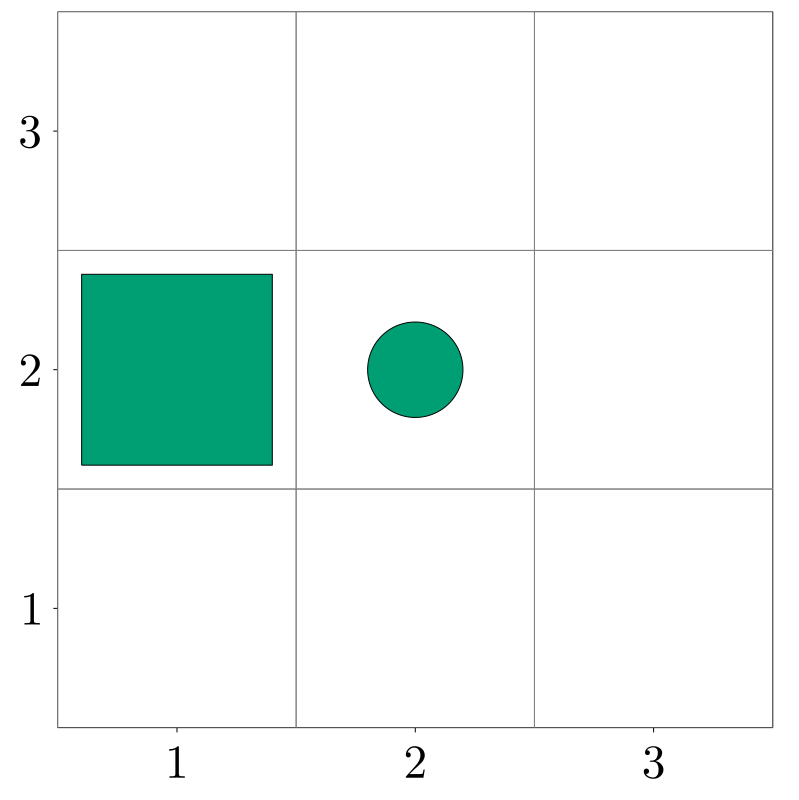
\includegraphics[width=4cm]{"./figures/s3.png"}} &,\ p=0.2 \\
          \parbox[h][0.3\linewidth][c]{0.25\linewidth}{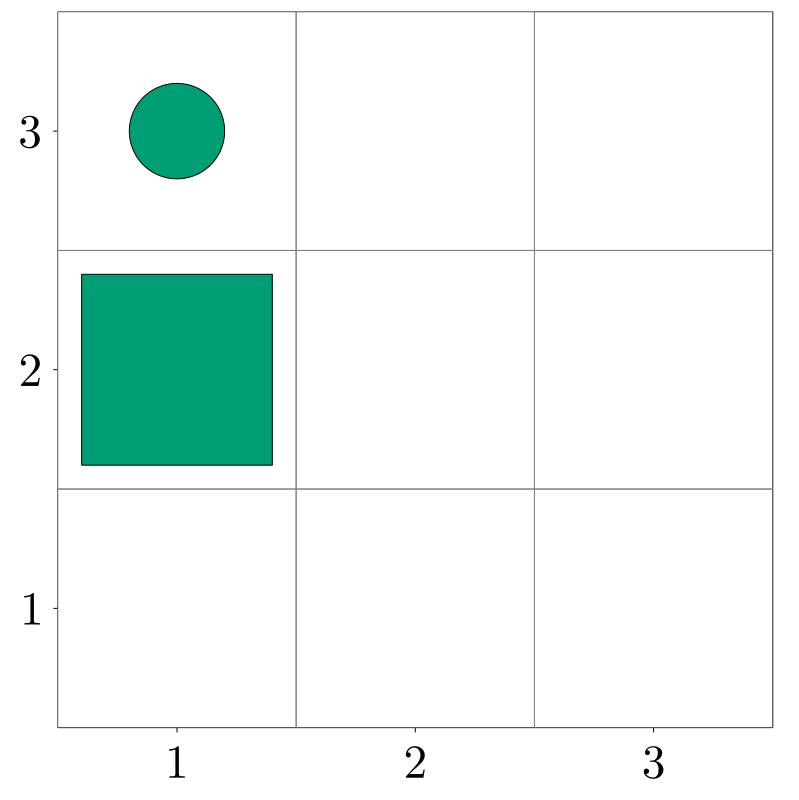
\includegraphics[width=4cm]{"./figures/s4.png"}} &,\ p=0.2 \\
          \parbox[h][0.3\linewidth][c]{0.25\linewidth}{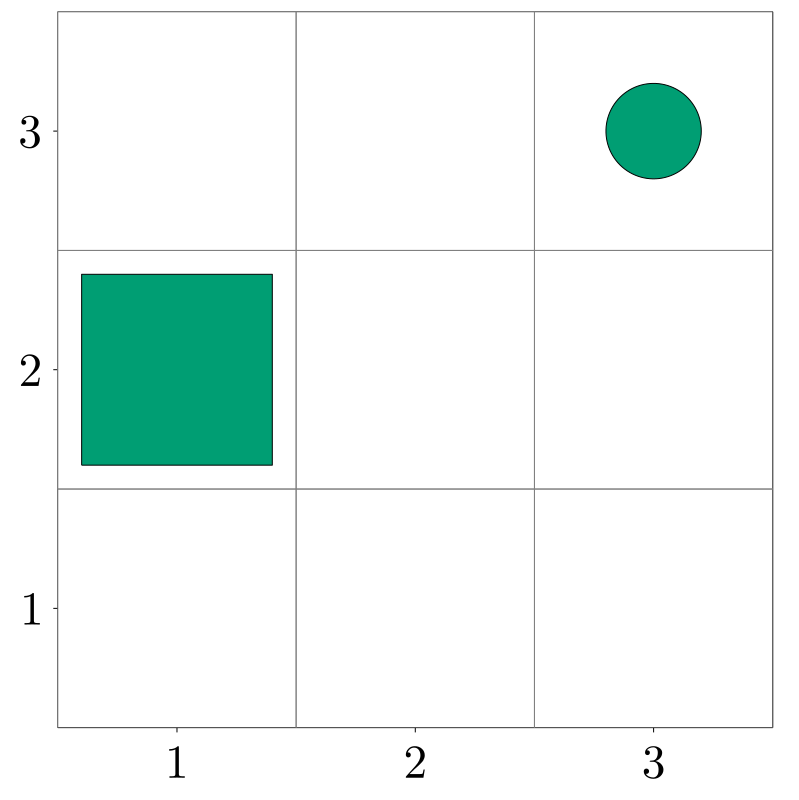
\includegraphics[width=4cm]{"./figures/s5.png"}} &,\ p=0.2 \\
          \end{tabular}
          % \end{align*}
          % }
    \right.
  \]
  \caption{Now in this figure we can see an example of a stochastic transition function. On the left hand side we can see the state $s_t$ and the action $a_t$. On the right hand side we can see the probability distribution over the future states and their corresponding probabilities. }
  \label{fig:stochastic_transition}
\end{figure}

\subsubsection{Partially observable grid world}
When we choose to extend the MDP to a POMDP we will do it by letting the agent only perceive a certain distance. For example the rectangle created by all the adjacent cells. In Figure \ref{fig:redline}, we can see this demonstrated. However, we can also extend it to include all the cells adjacent in two steps, and so on. 

\begin{figure}[H]
  \centering
  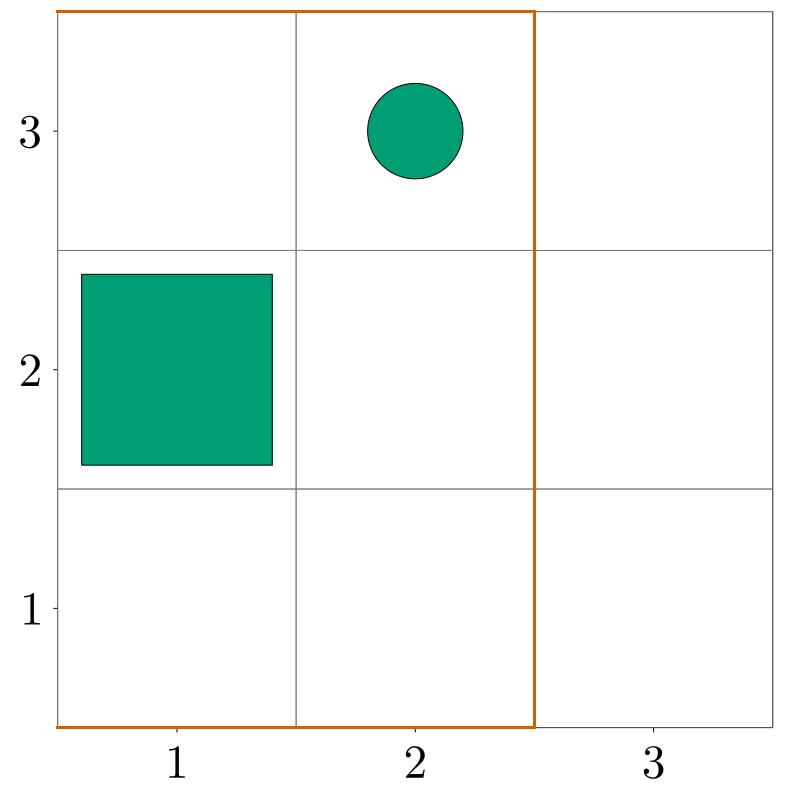
\includegraphics[width=4cm]{"./figures/s2_redline.png"}
  \caption{Here we can see a POMDP. The agent is represented by the green square and the observable part of the grid is all adjacent (both diagonally and direct) cells inside the orange line. }
  \label{fig:redline}
\end{figure}


\subsubsection{Including more foods}
In order to make the environment more complex we will be adding three different types of food, see Figure \ref{fig:multiple_foods}. The color of the agent represents which type of food the agent desires. The task thus becomes to consume a food which the agent has a desire towards. When the task is achieved the agent will get a new desire sampled from the set of possible desires, that is the possible colors of the food types. In Figure \ref{fig:multiple_foods} this set is \{blue, orange, green\}, and we can see on the right hand side that after consuming the green food type the new desire is blue. 
% Static vs Dynamic 
\begin{figure}[H]
  \centering
  \[
    T \left(
    \parbox[h][0.30\linewidth][c]{0.25\linewidth}{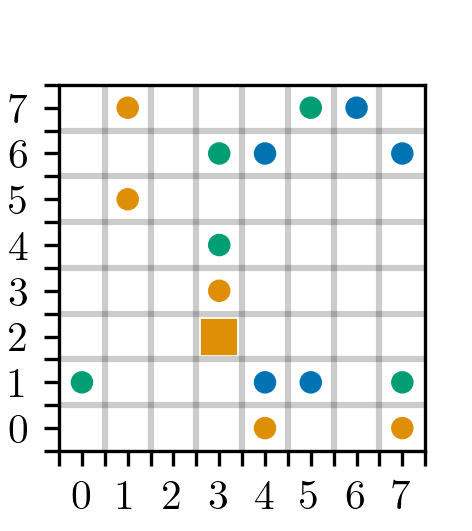
\includegraphics[height=4cm, width=4cm]{"figures/5x5.png"}}, \textit{UP} 
    \right)
    \sim \parbox[h][0.30\linewidth][c]{0.25\linewidth}{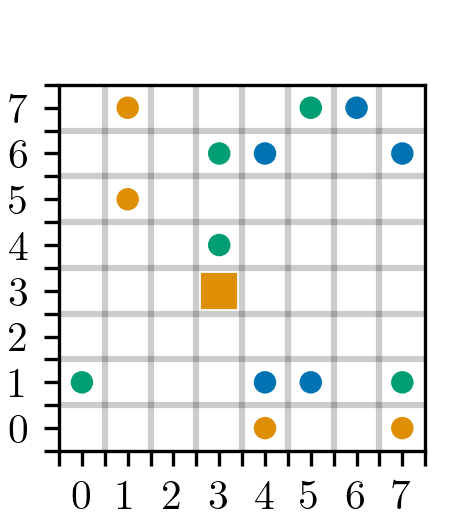
\includegraphics[width=4cm]{"./figures/5x5_2.png"}}
  \]
  \caption{Above we find a more complex grid which is inputted to its transitional function $T$ with the UP action. On the right hand-side we can see a new state drawn from the distribution which $T$ outputs.}
  \label{fig:multiple_foods}
\end{figure}

Now with multiple foods added to the environment, the agent consuming a food type it does not desire is possible. When this happens, we will consider it a side effect since consuming undesired food types does not help the agent consume the right food type, besides perhaps allowing a quicker path.


\subsection{Simulation}
To test how adding an impact measurement to our agent, we will train the agent in both a static and a dynamic grid world. The size of the grid world will be $10\times10$. Also, we will be adding that the agent will only be able to perceive cells two steps away from it, including diagonally, so it can perceive a $5\times5$ grid.

\begin{table}
  \centering
  \begin{tabular}{l | c}
    Parameter& Value \\ \hline
    grid size & $10 \times  10$ \\
    observation size & $5 \times  5$ \\
    $\gamma$ & 0.95 \\
    number of foods & 3 \\
    base reward & -0.04 \\
    food reward & 1 \\
    prob food move & 0 \\
  \end{tabular}
  \
  \begin{tabular}{l | c}
    Parameter& Value \\ \hline
    grid size & $10 \times  10$ \\
    observation size & $5 \times  5$ \\
    $\gamma$ & 0.95 \\
    number of foods & 3 \\
    base reward & -0.04 \\
    food reward & 1 \\
    prob food move & 1 \\
  \end{tabular}
  \caption{CAPTON}
  \label{tab:sim_parms}
\end{table}

\section{Agent}
We will train the agent using the PPO-algorithm described in the previous chapter. To include an impact measurement, we will modify the algorithm to consider future tasks, and this approach we will refer to as PPO-FTA. However, instead of simulating the availability of future rewards, we will use a second critic network to estimate the value function for other tasks. 

We will train the second critic network before the initialization of the PPO-FTA algorithm, and there are two significant differences in the training procedure. Firstly, the training distribution will be more diverse by including different amounts of foods initially. Secondly, to make the critic more general, we will also apply augmentations to the grids, such as changing the colors and rotating the grid. These augmentations are motivated by the fact that the estimated reward should be the same regardless of the colors since they all give the same reward. Furthermore, neither should the direction matter since the distance is the same regardless. 




%########################################################################%
% RESULTS
%########################################################################%

\chapter{Results}



%########################################################################%
% DISCUSSION
%########################################################################%

\chapter{Discussion}
% Self conciousness might be necessary to enable the agent to differentiate between side effects it caused and those who happened trough natural dynamics.

% Life is about a journey, not mazimizing goals, thus we should be happy with AI doing that for us. 

% consciousness, panpsychism and the philosophy of Mind - Lex Fridman #261, maybe better placen in an apendix

% Ad-hoc solutions to get performance on SafeLife, but improving scores on benchmarks can help the fiel ImageNet  
% https://www.eff.org/ai/metrics

% Partly observable and stochastic simulations to make more similar real world, multi agent


%########################################################################%
% CONCLUSION
%########################################################################%

\chapter{Conclusion}


% \printbibliography
\bibliography{ref}
\bibliographystyle{apalike}
% \printbibliography

\end{document}

\subsection{Solving MDP}
The policy $\pi$ includes what action to take in which states. A policy that only includes the optimal actions for each state is called the optimal policy and is denoted as $\pi^*$. The actions in the optimal policy $\pi^*$ yields the highest expected reward when executed. One solves an MDP by finding the optimal policy, there exists several methods for finding the optimal policy, but we are in this report going to use \textit{value iteration}. 
% solvable with the Bellman equation

To solve an MDP we begin with defining the \textit{Q-function},
\[ Q(s, a) = \sum_{s^\prime}p(s^\prime|s_t,a)[r(s_t,a,s^\prime) + \gamma U(s^\prime)],\]
which computes the expected reward when performing an action $a$ in state $s$, where $s^\prime$ denotes a possible future state. Here the reward is based on the \textit{utility}, this is defined as the expected reward with the action that maximizes the \textit{Q-function},
\begin{align*}
  U(s) =& \text{max}_{a\in \mathcal{A}(s)} \sum_{s_{t+1}}P(s_{t+1}|s_t,a)[r(s_t,a,s_{t+1}) + \gamma U(s_{t+1})]\\
  = &  \text{max}_{a\in \mathcal{A}(s)} Q(s,a)\\
\end{align*}

With the with the utility in each state, it is then possible to find the optimal policy from each state by selecting the action that yields the highest utility,
\[ \pi^*(s) = \text{argmax}_a Q(s,a) \]

Since computing the utility in one state requires the utility in other states, the computation is not straight forward. To solve this we can utilize a dynamic algorithm, in this report we will use \textbf{value iteration}. This algorithm is a iterative computation that is executed until a equilibrium is reached. The updating of the utility is called an \textbf{Bellman update} and looks like this,
\[U_{i+1}(s) \leftarrow \max_{a\in\mathcal{A}} \sum_{s\prime} p(s^\prime|s,a)[R(s,a,s^\prime) + \gamma U_i(s^\prime)].\]

